%File: icwsm2026-restructured.tex
\documentclass[letterpaper]{article} % DO NOT CHANGE THIS
\usepackage[submission]{aaai2026}  % DO NOT CHANGE THIS
\usepackage{times}  % DO NOT CHANGE THIS
\usepackage{helvet}  % DO NOT CHANGE THIS
\usepackage{courier}  % DO NOT CHANGE THIS
\usepackage[hyphens]{url}  % DO NOT CHANGE THIS
\usepackage{graphicx} % DO NOT CHANGE THIS
\usepackage{amsmath}
\usepackage{booktabs}
\urlstyle{rm} % DO NOT CHANGE THIS
\def\UrlFont{\rm}  % DO NOT CHANGE THIS
\usepackage{natbib}  % DO NOT CHANGE THIS AND DO NOT ADD ANY OPTIONS TO IT
\usepackage{caption} % DO NOT CHANGE THIS AND DO NOT ADD ANY OPTIONS TO IT
\frenchspacing  % DO NOT CHANGE THIS
\setlength{\pdfpagewidth}{8.5in} % DO NOT CHANGE THIS
\setlength{\pdfpageheight}{11in} % DO NOT CHANGE THIS
%
%\usepackage{algorithm}
%\usepackage{algorithmic}
%\usepackage{newfloat}
%\usepackage{listings}
\DeclareCaptionStyle{ruled}{labelfont=normalfont,labelsep=colon,strut=off} % DO NOT CHANGE THIS



\pdfinfo{
/TemplateVersion (2026.1)
}

\usepackage{xcolor}
% Define a command for each author
\newcommand{\cb}[1]{\textcolor{blue}{CB: #1}}
\newcommand{\ml}[1]{\textcolor{red}{ML: #1}}
\setcounter{secnumdepth}{2}

\title{Depth, Breadth, and Bias: Structural Diffusion of Political Content on Divergent Platforms}
\author{
    Written by AAAI Press Staff\textsuperscript{\rm 1}\thanks{With help from the AAAI Publications Committee.}\\
    AAAI Style Contributions by Pater Patel Schneider,
    Sunil Issar,\\
    J. Scott Penberthy,
    George Ferguson,
    Hans Guesgen,
    Francisco Cruz\equalcontrib,
    Marc Pujol-Gonzalez\equalcontrib
}
\affiliations{
    \textsuperscript{\rm 1}Association for the Advancement of Artificial Intelligence\\
    1101 Pennsylvania Ave, NW Suite 300\\
    Washington, DC 20004 USA\\
    proceedings-questions@aaai.org
}

% REMOVE THIS: bibentry
\usepackage{bibentry}
% END REMOVE bibentry

\newcommand{\answerTODO}[1]{#1}
% ---- Revision highlighting: text added or changed in the R&R revision ----
\usepackage{xcolor}
\usepackage{booktabs}
\newcommand{\rev}[1]{{\color{blue}#1}}
% --------------------------------------------------------------------------
\begin{document}

\maketitle

\begin{abstract}

When political content spreads on social media, does diffusion follow universal structural patterns or are these patterns shaped by platform-specific communities? We address this question by comparing how cascades during the 2024 U.S. presidential campaign scale on two ideologically distinct but technically comparable platforms: Truth Social and Bluesky. Using repost and reply networks constructed from public posts mentioning Biden or Trump (May–June 2024), we examine whether similarly sized cascades take similar shapes across platforms. We find that amplification (reposts) scales similarly. Conversational diffusion, however, diverges sharply: reply cascades on Truth Social are wider and shallower, while those on Bluesky are narrower and deeper. We evaluate candidate explanations: influencer dominance, topic variability, ideological composition, and cross-ideological interaction alignment. Neither influencers nor topic differences account for this divergence. Only when both ideological composition and interaction alignment are modeled together do platform-level scaling differences effectively disappear. 
Fine-grained motif analysis further reveals asymmetric interaction patterns, including distinct roles for left-, right-, and center-leaning users across platforms. Overall, the findings show that platform differences matter most where political diffusion becomes conversational. Our paper highlights that next-generation social media platforms do not simply transmit political information at different volumes; they organize different opportunities for political engagement and disagreement across ideological groups.

\end{abstract}


\section{Introduction}
Social media platforms facilitate information cascades, reposts, replies, and other interactions through which political content circulates online \cite{easley_networks_2010, gruhl_information_2004, guille_information_2013}. 
%Understanding how these cascades form has become a central concern across computational social science, communication, and network analysis. 
A central question in computational social science is whether the structural patterns of these cascades are governed by universal dynamics or shaped by the particular environments in which they unfold. While there is past work on how diffusion structures vary across information types (e.g., false vs. real news~\citep{vosoughi_spread_2018}), 
we know little about how diffusion scaling properties vary across platforms.
%most past scholarship focuses on a single platform. This limits what we know about which aspects of diffusion are universal and which are platform-specific, especially in newer, ideologically distinct online environments \cite{cinelli_echo_2021}.
%\cb{i feel like this is more of a related work material, i tried to reformulate it above a little. feel free to work in the citations i skipped, i cant remember which of those  were doing comparative and comparison across what.}
%Past research has shown how different types of content, such as videos, petitions, or news, spread on platforms including Twitter, Facebook, and LinkedIn, and how false news in particular can diffuse differently than true news \cite{goel_structural_2016, cheng_can_2014, anderson_global_2015, vosoughi_spread_2018, zhao_fake_2020}.

%\cb{again, i feel like this is more for related work. here you are making the reader think of design vs community but we dont really answer the question of which one. one way you can work this in is maybe adding one more sentence at the end of the first saying "there are good reasons to expect platform level differences, affordance <cites>, communities<cite>. But do they emerge?" I leave it to you to decide or move this to the related work}
%Much of this work highlights two broad influences. First are platform affordances, features like reply visibility, feed ranking, or sharing mechanisms, that determine what users see and how they can interact \cite{boyd_social_2010, treem_social_2013}. Second are community dynamics: who participates, how like-minded or diverse those users are, and whether they engage across ideological boundaries \cite{conover_political_2011, garimella_political_2018}. These factors together shape whether cascades remain shallow amplifications or develop into extended conversations.

%Existing studies have often aggregated cascades by content type (e.g., true vs. false news) and examined size, depth, breadth, or virality to identify broad drivers such as novelty, veracity, or emotional tone \cite{goel_structural_2016, vosoughi_spread_2018, berger_what_2012, zollo_emotional_2015}. However, most analyses focus on a single platform, limiting what we know about which aspects of diffusion are universal and which are platform-specific, especially in newer, ideologically distinct online environments \cite{cinelli_echo_2021}.

This question has become increasingly relevant because the social media ecosystem has fractured. After the January 6 Capitol attack, Donald Trump launched Truth Social as a right-leaning alternative to mainstream platforms. More recently, Twitter's rebranding as X and its loosening of moderation have spurred many centrist and left-leaning users to migrate to Bluesky \cite{gerard_truth_2023, failla_im_2024, quelle_bluesky_2024}. Although both platforms mimic Twitter's design, follower networks, reposts, and reply mechanics, their contrasting community compositions create distinct social contexts. 
This creates a natural testbed to determine whether similar technical designs produce similar diffusion structures when embedded in different communities.
%Prior studies of Gab, a platform built to closely mimic Twitter's technical design, show that similar architectures can foster very different conversational structures when embedded in different communities \cite{cinelli_echo_2021}.

To answer this question, we compare the structural diffusion of political content on Truth Social and Bluesky during a high-salience period of the 2024 U.S. presidential campaign. The analysis centers on a one-month window that included major events such as the first presidential debate, focusing on posts containing hashtags and keywords related to ``Biden'' and ``Trump.'' 
To characterize diffusion dynamics, we go beyond raw comparisons of cascade size, depth, or breadth. Such comparisons across platforms can be misleading since platforms with more users mechanically generate larger cascades~\citep{juul_comparing_2021}. Instead we focus on how cascades grow as they scale. We compute scaling to determine whether each additional participant tends to broaden a cascade horizontally or deepen it vertically on a given platform. If scaling relationships are platform-specific, identical levels of engagement produce fundamentally different conversational geometries. Our goal is to understand if such divergence happens and why.

When performing cross-platform comparisons, we also distinguish between diffusion modes. Reposts and replies serve different functions: reposts are acts of amplification that redistribute content to new audiences, while replies are conversational acts that extend, contest, or elaborate on content~\citep{conover_political_2011,boyd_tweet_2010,guerrero_sole_interactive_2018}. Past work has identified important distinctions between these diffusion modes, such as differences in homophily~\citep{conover_political_2011}. However, cascade research typically aggregates both into general engagement metrics. By treating repost and reply cascades as distinct objects, we can test whether cross-platform universality holds for amplification, for conversation, or for both.

%Truth Social and Bluesky provide a natural comparison for studying how candidate-related political conversations unfold in ideologically distinct online environments. Rather than emphasizing only how far or how fast information travels, our analysis focuses on the shapes of cascades: whether content spreads broadly through direct amplification or develops sequentially through extended exchanges.

%Building on this insight, we compare the structural diffusion of political content on Truth Social and Bluesky during a high-salience period of the 2024 U.S. presidential campaign. The analysis centers on a one-month window that included major events such as the first presidential debate, focusing on posts containing hashtags and keywords related to ``Biden'' and ``Trump.'' We ask: Which aspects of diffusion are consistent across platforms, and which vary with community composition and interaction norms?

We find that platform differences matter most where political diffusion becomes conversational. Repost cascades scale similarly across Truth Social and Bluesky. %, suggesting that sharing-based amplification may scale in comparable ways across technically similar platforms. 
Reply cascades, by contrast, diverge sharply: Truth Social produces wider and shallower interactions, while Bluesky produces narrower and deeper conversational threads. 

What explains these fundamental differences? Platforms can vary in the dominance of their influential users and this can impact diffusion patterns~\citep{goel_structural_2016, zannettou_what_2018}. 
%Indeed, Truth Social was launched by Donald Trump, who continues to play a significant role on the platform~\citep{pew_truthsocial_2022}. 
Similarly, certain topics can be more contentious, leading to different diffusion patterns \cite{vosoughi_spread_2018, wang_factors_2022} and topic distribution can vary across platforms. Interestingly, we find neither of these explain the reply scaling differences between the two platforms. Ideological composition partially explains the differences and, most importantly, when accounting for both composition and the degree to which users engage in cross-ideological discussions, the platform level differences disappear. 

Motif analysis helps unpack what this aggregate alignment pattern means locally. It shows that cross-ideological interaction takes different structural forms across platforms: on Truth Social, disagreement more often appears as parallel replies around the same parent post, whereas on Bluesky it more often appears as sequential chains that extend conversations across turns.

%These differences are explained more strongly by ideological composition and interaction alignment than by influencers or topic variation.

These findings matter for understanding the fragmented social media ecosystem. Newer platforms are often built around familiar Twitter-like features, but similar technical designs do not guarantee similar political interaction. Our findings show that political information can be amplified in similar ways while being discussed in very different ways, with replies revealing how platform communities organize opportunities for ideological engagement, disagreement, and visibility.

\section{Related Work}

\subsection{Comparative Cross-Platform Analysis}


A growing body of research argues that social media should be studied as a fragmented ecosystem of platforms rather than as a single, unified public sphere \cite{rowe_mining_2014, boulianne_engagement_2023}. Comparative work shows that political ideology predicts both platform adoption and political use, while platform-specific networking features shape what kinds of political exposure and expression occur there \cite{boulianne_social_2025}. At the ecosystem level, recent scholarship suggests that online fragmentation increasingly takes the form of ``echo platforms,'' in which ideological differentiation emerges not only within platforms but between them as users migrate across services with distinct moderation regimes, recommendation logics, and community norms \cite{di_martino_ideological_2025,  mosleh_crossplatform_2025}.

This perspective is especially important for the study of alternative and emerging platforms. Research on Gab established early that alt-tech platforms can attract ideologically concentrated user bases and sustain different information environments from those observed on mainstream sites \cite{zannettou_what_2018}. More broadly, \citet{cinelli_echo_2021} show that homophilic clustering and like-minded information diffusion vary substantially across platforms, indicating that similar affordances do not guarantee similar interaction dynamics. Their comparison of Facebook, Twitter, Reddit, and Gab underscores the importance of platform-specific interaction environments in shaping information exposure and segregation.

Work on Truth Social remains comparatively sparse, but existing studies already suggest that it is best understood as a politically concentrated alt-tech environment rather than simply a new campaign tool. Early dataset work positioned Truth Social as a refuge for users alienated by mainstream moderation and documented its rapidly emerging network and content ecology \cite{gerard_truth_2023}. Subsequent work released a large 2024 election dataset with posts, replies, and user interactions, emphasizing the platform's role in hosting contentious, often hyper-partisan political discourse \cite{shah_unfiltered_2024}. More recent network analysis similarly characterizes Truth Social as ideologically homogeneous and structurally segmented, with attention concentrated around a small set of central actors \cite{hughes_truthsocial_2025}.

By contrast, recent work on Bluesky describes a Twitter-like platform with a markedly different political center of gravity. Early studies characterized Bluesky as an emerging alternative to X and documented its rapidly expanding data ecology, including large-scale post histories, follow relations, replies, reposts, quotes, and feed-generator interactions \cite{failla_im_2024}. More recent work shows that Bluesky exhibits heavy-tailed, highly clustered network structure similar to larger platforms, but that users share predominantly left-center news sources and make limited use of custom algorithmic feeds \cite{quelle_bluesky_2024}. \citet{nogara_bluesky_2026} further find that Bluesky maintains relatively high levels of original posting, low toxicity, and high-credibility news sharing even after rapid growth following its public launch. Together, these studies position Truth Social and Bluesky as a valuable comparative pair: technically comparable platforms embedded in sharply different ideological communities.

%Our study builds on this comparative tradition by shifting the focus from platform adoption, content quality, or partisan composition alone to the structural geometry of diffusion. Rather than asking only what kind of political content circulates on each platform, we ask whether similar affordances produce similar cascade forms, and whether divergence emerges more clearly in amplification-oriented interactions such as reposts or in conversational interactions such as replies.


\subsection{Information Diffusion and Cascade Structure}


Research on information diffusion has developed a rich vocabulary for describing how online content spreads through networks, including cascade size, depth, breadth, and structural virality \cite{gruhl_information_2004, guille_information_2013, easley_networks_2010, goel_structural_2016}. This literature has linked cascade structure to content attributes such as veracity, novelty, emotional tone, and topic salience. Most prominently, \citet{vosoughi_spread_2018} show that false news on Twitter spreads farther, faster, deeper, and more broadly than true news. Further work examines how topic salience~\cite{wang_factors_2022}, cascade predictability~\cite{cheng_can_2014}, and misinformation propagation~\cite{zhao_fake_2020} shape diffusion.

A related development concerns interaction type. Diffusion studies often prioritize reposting or retweeting because these traces are easy to reconstruct and map directly onto dissemination. Reposting is especially important for political amplification: experimental evidence from Facebook shows that reshared content substantially increases exposure to political news and low-quality sources, demonstrating the centrality of reshare mechanisms to political visibility \cite{guess_reshare_2023}. Foundational work on retweeting also shows that reposts are socially meaningful acts of redistribution, attribution, and audience management, rather than neutral transmission alone \cite{boyd_tweet_2010, park_expanding_2019}. 

Yet reposting is only one mode of information flow. Prior work shows that retweets, mentions, replies, and quote tweets capture different forms of political engagement. In U.S. election discourse, retweet networks are highly segregated by ideology, whereas mention networks are more politically heterogeneous and contain more cross-ideological interaction \cite{conover_political_2011}. Studies of political discussions similarly treat retweeting, mentioning, and replying as distinct behavioral traces, with retweet networks more likely to resemble echo chambers and replies or mentions more likely to reflect direct interaction \cite{guerrero_sole_interactive_2018}. Other work finds that emotional and textual features affect replies and retweets differently, suggesting that response-oriented conversation and amplification-oriented redistribution follow different behavioral logics \cite{kim_role_2012, toraman_understanding_2022}. Finally, studies of threaded political conversations show that replies can sustain extended argument across ideological divides, making reply trees especially useful for studying conversational engagement rather than simple visibility \cite{shugars_why_2019}.

%This distinction remains underdeveloped in cascade research, where reposts and replies are often folded into general measures of engagement or studied separately without a common structural framework. Our study builds on this work by treating repost and reply trees as distinct cascade objects. This allows us to test whether cross-platform similarities are concentrated in amplification-oriented diffusion, while platform-specific differences emerge more strongly in conversational diffusion.


\subsection{Ideology, Polarization, and Political Communication Online}


A large literature shows that online political communication is shaped by ideological homophily, selective exposure, and asymmetric cross-group engagement \cite{adamic_political_2005, conover_political_2011, flaxman_filter_2016, del_vicario_echo_2016}. Yet this work also suggests that different interaction types produce different political structures. \citet{conover_political_2011} show that retweet networks are highly segregated, whereas mention networks are more politically heterogeneous. Similarly, \citet{barbera_tweeting_2015} find that political communication often remains ideologically clustered, but that liberals are more likely than conservatives to engage in cross-ideological dissemination. These studies suggest that exposure to disagreement is unevenly distributed and depends in part on how users interact.

More recent work complicates any simple equation of cross-cutting exposure with deliberative benefit. \citet{bail_exposure_2018} show that following opposing political elites on social media can increase polarization rather than reduce it. \citet{garimella_political_2018} further identify gatekeepers and the ``price of bipartisanship,'' showing that users who bridge polarized communities often occupy structurally costly positions. In parallel, \citet{rathje_outgroup_2021} demonstrate that out-group animosity is a strong driver of sharing, implying that cross-ideological interaction on social media is often conflictual rather than integrative.

Recent evidence also points to ideological asymmetries in what gets diffused. \citet{chang_share_2025} show that liberals and conservatives differ in the range of issues and the toxicity of elite content they retransmit, suggesting that downstream information environments are shaped not only by whom users follow, but also by what kinds of content each side disproportionately passes along. This raises a related question for cascade analysis: whether political structure operates mainly through user composition, through the alignment of interactions within and across groups, or through both at once.

%Our study extends this literature by distinguishing between ideological composition and interaction alignment as separate mechanisms. Composition captures who is present in a cascade; alignment captures whether interactions are concentrated within ideological groups or cut across them. By examining how these factors mediate breadth and depth in reply cascades, and by comparing their roles across repost versus reply trees, we connect classic questions of homophily and polarization to the structural analysis of diffusion.

\subsection{Theoretical Framework and Hypotheses}

\subsubsection{Defining Diffusion Modes and Scaling.}
As we mentioned before, we distinguish between two modes of diffusion: reposts and replies. Rather than emphasizing only how far or how fast information travels, our analysis focuses on the shapes of cascades: whether content spreads broadly through direct amplification or develops sequentially through extended exchanges. Prior work has shown that depth, breadth, and structural virality all correlate positively with cascade size \cite{juul_comparing_2021}. This raises a concern: marginal comparisons may conflate structural effects with sheer volume. To address this, we hold cascade size constant and examine structural differences directly, analyzing how cascades grow vertically (depth) and horizontally (breadth).


This scaling perspective leads to a broader question: when cascades reach similar sizes, do they take similar structural forms across platforms and diffusion modes, or do they grow through different geometric patterns? If diffusion scaling is broadly universal, similarly sized cascades should exhibit comparable depth and breadth regardless of platform. If scaling is platform-specific, then the same level of participation may produce different cascade shapes depending on the interaction environment.

We therefore examine three candidate explanations for cross-platform variation in cascade geometry. First, user prominence may shape scaling if highly followed or highly active users attract many direct interactions, producing broader cascades. Second, topic variability may matter if some topics invite rapid amplification while others encourage extended discussion. Third, ideological composition and interaction alignment may shape scaling by affecting whether interactions remain within like-minded groups or extend across ideological boundaries. 

\subsubsection{H1: Influencer Dominance.}
Prior research has demonstrated that a small number of high-follower users can disproportionately influence content dissemination, particularly on platforms characterized by skewed follower distributions \cite{goel_structural_2016, zannettou_what_2018}. Truth Social, with its relatively small and ideologically concentrated user base, offers a fertile environment for such dynamics. This is supported by power-law distributions in followers, reposts, and replies per user (see Appendix~\ref{app:powerlaw}), where Truth Social exhibits a more pronounced heavy-tailed distribution than Bluesky, with a handful of dominant accounts occupying central roles. A clear discontinuity separates the top eight users from the rest, providing a natural cutoff for defining unusually high influence. We hypothesize that this concentration contributes to reply cascades that are broad but shallow, indicative of immediate visibility rather than sustained conversational engagement.

\subsubsection{H2: Ideological Structure.}

The ideology of users in a cascade may shape its structure through both participation and interaction. Prior work shows that online political interaction is strongly structured by ideological homophily and selective exposure: amplification networks are often more segregated, while more conversational channels can include greater cross-ideological contact \cite{conover_political_2011, garimella_political_2018, barbera_tweeting_2015, adamic_political_2005, guess_how_2023}. However, this literature does not directly establish how ideological alignment affects cascade geometry. We build on it by asking whether ideological composition and cross-ideological interaction are associated with how reply cascades scale in depth and breadth.

We measure ideological structure along two dimensions: (1) \textit{ideological composition}, defined as the proportion of users from each stance within a reply tree, and (2) \textit{interaction alignment}, defined as the share of reply edges connecting users with the same ideological label. Lower alignment indicates more cross-cutting interaction. As shown later in Appendix~\ref{app:ideology_distribution}, Truth Social and Bluesky differ substantially in the ideological composition of their observed users, making ideological structure a plausible source of cross-platform differences in reply geometry.

We hypothesize that ideological composition and interaction alignment play a significant role in how reply cascades scale. If cross-platform differences in cascade geometry are driven by ideological structure, then incorporating composition and alignment into the models should substantially attenuate platform-level differences in depth and breadth.

\subsubsection{H3: Topic Variability.}
Post content shapes how users interact with it. Emotionally charged, controversial, or conspiratorial content often spreads through deeper and more structurally viral cascades than neutral or factual information \cite{vosoughi_spread_2018, wang_factors_2022}. As described in Section~\ref{sec:topicmodel}, we identified eleven salient topics across both platforms; while all are politically related, their distribution differs substantially between Truth Social and Bluesky. We hypothesize that topics play a significant role in how diffusion dynamics scale on social media. For instance, topics involving partisan conflict, institutional distrust, or election-related narratives may elicit distinct structural diffusion patterns depending on their resonance within each platform's community. 

\subsubsection{Micro-Level Network Motifs.}
To unpack the mechanisms behind platform-level differences in reply cascade geometry, we complement cascade-level regressions with motif analysis, a graph-theoretic approach examining the frequency of small recurring substructures within larger networks~\cite{alon_network_2007}. While statistical models evaluate whether alignment ratio and ideological composition explain divergence, they do not reveal \textit{how} these compositional factors shape micro-dynamics of interaction. We analyze two basic 3-node motif shapes: \textit{chains}, where replies unfold in sequence, and \textit{stars}, where multiple replies attach to the same root. Each motif is labeled by the ideological stance of its participants: Left (L), Center (C), or Right (R).


\section{Data and Methods}

\subsection{Data Collection}
We collected posts and their associated reposts and replies from both platforms during a critical month of the 2024 U.S. presidential campaign, when major political events (including the first debate) spurred intense online discussion. We used each platform's public API to collect posts containing the target keywords and their surrounding conversations. For Bluesky, the thread endpoint enabled retrieval of entire discussion trees around posts mentioning ``Biden'' or ``Trump,'' while for Truth Social (which follows the Mastodon API structure), we used the context endpoint to capture both ancestor and descendant replies recursively. This approach provides full conversational context rather than isolated messages, allowing us to reconstruct entire reply cascades. For every post and reply, we also collected associated repost actions and each user's follower list. Data were collected between May 30 and June 30, 2024, a high-salience period that included the first U.S. presidential debate.

\subsection{Cascade Construction}
We model information diffusion as directed acyclic graphs (DAGs), where \rev{each node is a single post (the root post, a reply, or a repost)} and edges represent inferred diffusion pathways, following the time-inferred approach of \citet{vosoughi_spread_2018}. \rev{Nodes are posts rather than accounts, so a user who replies several times in one thread contributes one node per reply. Ideology, by contrast, is aggregated at the user level: each node carries the label of the account that wrote it (see Ideology Estimation and Alignment), so a cascade's ideological composition is the share of its posts written by left- or right-leaning accounts.} For \textbf{reply cascades}, trees were constructed directly from reply metadata: each reply is linked to its parent post, and cascades are rooted at the original post with subsequent replies linked recursively. For \textbf{repost cascades}, platform APIs report all reposts as nominally linking to the original post, which obscures the true diffusion path. To approximate true repost trees, for each repost $r_i$ we identified all prior reposts $r_j$ with $t_j < t_i$ such that $r_i$ \rev{is observed to follow the user who made $r_j$ in the follower snapshot}, then inferred the edge $r_j \rightarrow r_i$ linking each repost to the most recent eligible prior repost. When no such user existed, the repost was attributed directly to the original post. This procedure infers the most probable diffusion paths based on temporal and social proximity. \rev{Because these edges are inferred rather than observed, we refer to repost cascades as reconstructed throughout, and we verify that the repost results are invariant to the reconstruction rule (Appendix, Robustness of Repost Cascade Reconstruction). Reconstruction assumptions can distort cascade properties \citep{deverna_cascade_2024}, so we assess whether the substantive conclusions are robust across several alternative rules. The follower network is a post-collection snapshot without edge creation dates, and was collected at the same time for both platforms.}

\subsection{Cascade Metrics}
For each cascade we compute four structural metrics. \textbf{Size} ($N$) is the \rev{total number of posts in the cascade, including the root}. \textbf{Breadth} ($B$) is the maximum number of nodes at any single depth level: $B = \max_{d \geq 1} n(d)$, where $n(d)$ is the node count at depth $d$. This captures the widest ``layer'' of the cascade and differs from root out-degree, which counts only direct children of the root. \textbf{Depth} ($D$) is the maximum hop distance from the root to any leaf node: $D = \max_{v} \mathrm{dist}(\mathrm{root}, v)$. \textbf{Structural Virality}~\cite{goel_structural_2016} is the average pairwise shortest-path distance between all nodes in the cascade, distinguishing broadcast-like (low virality) from chain-like viral (high virality) spread. All metrics were log-transformed for modeling due to heavy-tailed distributions.
\begin{figure*}
    \centering
    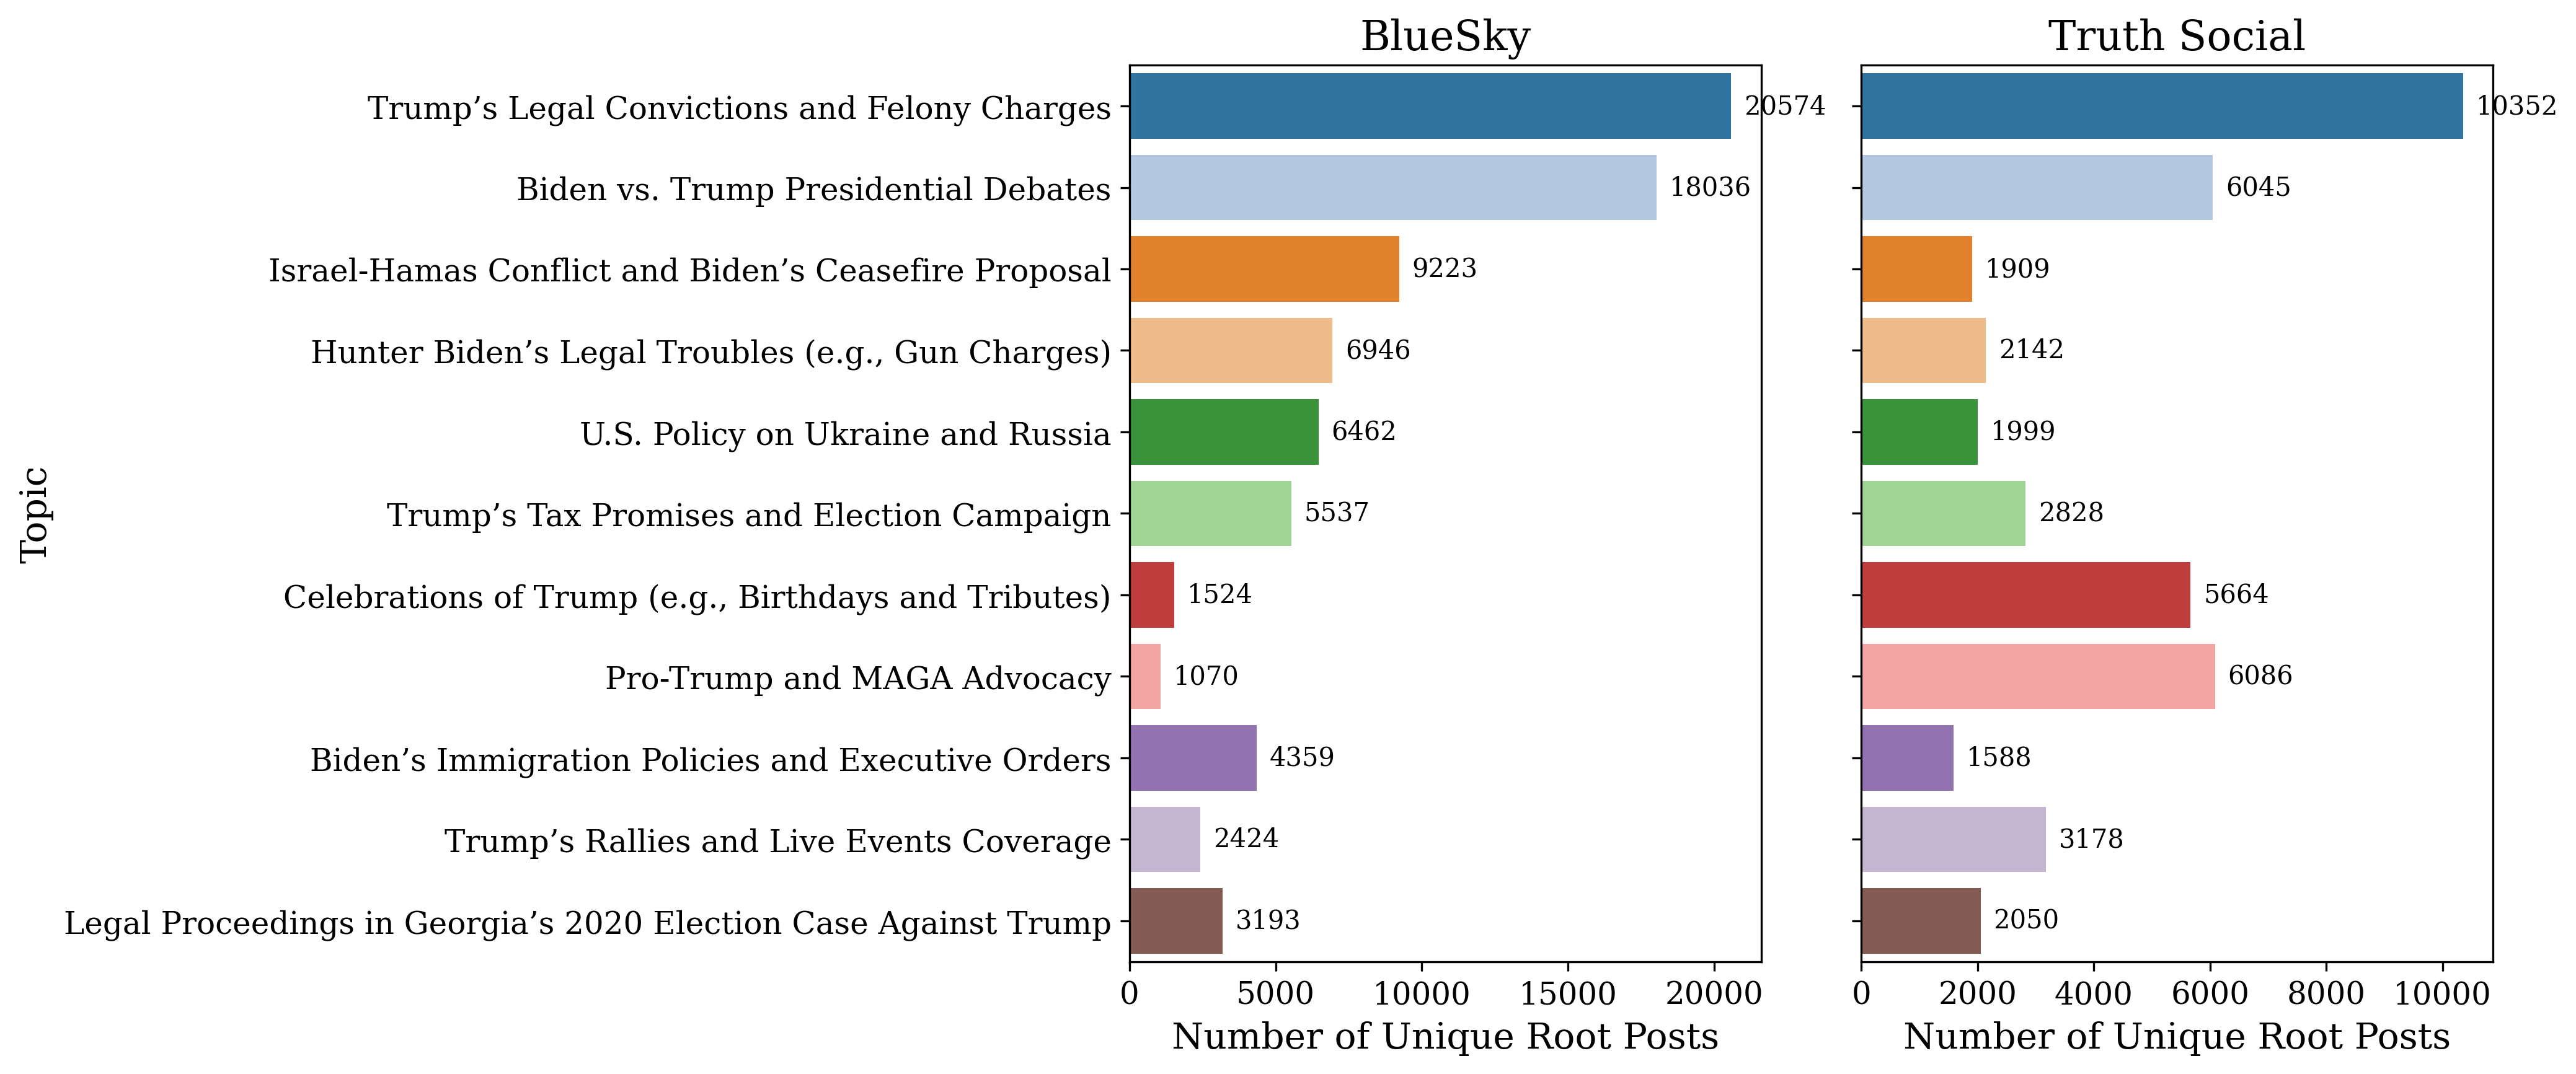
\includegraphics[width=\linewidth]{figures/topic_dis.png}
    \caption{Topic distribution across \textit{Bluesky} and \textit{Truth Social}.  
Bar plots show the number of unique root posts assigned to each of the 11 topics, based on BERTopic clustering and manual labeling.}
    \label{fig:topic_dis}
\end{figure*}
\subsection{Topic Modeling}
\label{sec:topicmodel}
To identify dominant themes and evaluate H3, we applied BERTopic, which integrates contextual sentence embeddings (\texttt{all-mpnet-base-v2}), UMAP dimensionality reduction, and HDBSCAN clustering. Topics were extracted using class-based TF-IDF over a preprocessed vocabulary. Two human annotators independently reviewed a sample of representative posts from each cluster to produce consensus-based labels, yielding eleven coherent topic categories (inter-annotator $\kappa = 0.53$; model--Human 1 $\kappa = 0.67$; model--Human 2 $\kappa = 0.67$). Posts not assigned to any cluster were excluded from topic analyses. While both platforms engage heavily with Trump's legal cases and the 2024 election, Bluesky posts are more concentrated around policy and legal accountability, whereas Truth Social emphasizes celebratory or pro-Trump content (see Figure~\ref{fig:topic_dis}).



\subsection{Ideology Estimation and Alignment}

\paragraph*{Post-Level Stance Detection.}
We used the \texttt{Llama-3.1-8B-Instruct} model to classify each reply into one of five ideological stances (\textit{left}, \textit{lean-left}, \textit{center}, \textit{lean-right}, \textit{right}), providing the original post and preceding replies as context. For robustness, we grouped stances into three categories: \textit{left-leaning} (left, lean-left), \textit{center}, and \textit{right-leaning} (lean-right, right). Annotations were validated against two human annotators on a random sample of 200 replies\rev{: inter-annotator agreement was $\kappa = 0.77$ and model--human agreement $\kappa = 0.61$ and $0.74$, with class-specific and platform-specific performance and bootstrap intervals reported in Appendix Table~\ref{tab:validation}, together with an analysis showing that the results below are unchanged when labels are randomly corrupted at the measured error rates}. Because large language models may encode biases, we treat these labels as probabilistic indicators rather than ground truth.

\paragraph*{User-Level Ideology Inference.}
User ideology was inferred by aggregating stance labels across all posts authored by each user. A user was classified as \textit{left-leaning} if more than 60\% of their posts were labeled left or lean-left, \textit{right-leaning} if more than 60\% were labeled right or lean-right, and \textit{center} otherwise. \rev{The center category is therefore a residual: it collects users who reach neither threshold, mixing genuinely moderate users, users who post about politics inconsistently, and users whose stance the classifier could not resolve. Appendix section on the center category reports how the results change when composition and alignment are computed over partisan users only.} This threshold balances ideological signal with label consistency; aggregate patterns are robust across thresholds from 0.5 to 0.7 (see Appendix~\ref{app:ideology_distribution}). 

%The resulting platform-level distributions are also consistent with prior evidence on the political composition of these platforms: Truth Social has been shown to contain a large share of right-leaning or pro-Trump prominent accounts, while Bluesky users and news influencers are disproportionately left-leaning \cite{pew_truthsocial_2022, pew_bluesky_influencers_2025, pew_socialmedia_use_2025}. \cb{i think the ability to show truthsocial is more rightleaning vs bluesky more left wont be as impressive. but if i remember correctly, percentages identified were similar to each other. i would give more specific numbers. looking at the pew report, it seems to me the 1/6 ration for truth social is aligned but not sure about bluesky. i might be missing something.}

\paragraph*{Alignment Ratio.}
For each reply edge, we code it as \textit{aligned} if both users share the same ideology and \textit{misaligned} otherwise. The alignment ratio for a cascade is the proportion of aligned reply edges. High ratios indicate ideologically homogeneous discussions; lower ratios reflect cross-cutting exchanges. \rev{In this scenario, consider a thread with four replies: a right-leaning user replies to a right-leaning root author, a second right-leaning user replies to the same root, a left-leaning user replies to the root, and that left-leaning comment draws a reply from a right-leaning user. Three of the four edges connect users who share a stance and one crosses stances, so the alignment ratio is $3/4 = 0.75$. The measure is a property of the conversation rather than of any participant: the same user contributes aligned edges in one thread and crossing edges in another.} 

\subsection{Statistical Modeling}

\paragraph*{Baseline Model.}
To rigorously assess how cascade structure varies across platforms, we model the scaling relationship between cascade size and breadth using robust regression with the Huber loss function. This approach mitigates the influence of outliers, common in heavy-tailed cascade data, and addresses heteroskedasticity in residuals (see Appendix~\ref{app:strategy} for diagnostics).

Our baseline model examines how cascade breadth and depth scale with size, conditional on platform, including a platform indicator and its interaction with log-transformed cascade size:

\begin{align}
\label{eq:eq1}
\log(Y_i) =\ & \beta_0 + \beta_1 \log(\text{size}_i) \notag \\
             & + \beta_2 \cdot \text{platform}_i \notag \\
             & + \beta_3 \cdot \left( \log(\text{size}_i) \times \text{platform}_i \right) + \varepsilon_i ,
\end{align}
where $Y_i$ denotes either cascade breadth or depth. The coefficient of interest is $\beta_3$, which captures whether the relationship between cascade size and breadth differs by platform.

To quantify the explanatory contribution of additional covariates, we track percent attenuation of $\beta_3$:

\begin{equation}
\Delta = 1 - \frac{\hat{\beta}_{3,\text{aug}}}{\hat{\beta}_{3,\text{base}}} ,
\end{equation}

where $\hat{\beta}_{3,\text{base}}$ is the interaction coefficient from Eq.~\ref{eq:eq1} and $\hat{\beta}_{3,\text{aug}}$ is the corresponding estimate from augmented specifications (Models 2--4). A larger $\Delta$ indicates that added covariates account for a greater portion of cross-platform difference.

\paragraph*{Incorporating Influencer Dynamics.}
To evaluate H1, we extend the platform variable to three categories: 0 for Bluesky, 1 for Truth Social cascades initiated by non-influencers, and 2 for those initiated by the top eight high-follower users on Truth Social. No comparable concentration of outlier accounts exists on Bluesky.

\paragraph*{Assessing Ideological Composition and Alignment Effects.}
Building on user-level ideology labels, we include alignment ratio (spline-transformed, df\,=\,3, to capture nonlinear effects at extremes of homogeneity) and the proportions of left- and right-leaning users per reply tree (with a spline for the left-user ratio and a linear term for the right-user ratio, based on partial-residual diagnostics; see Appendix~\ref{app:spline}). Both measures are interacted with cascade size and platform indicators. We decompose this into three specifications: composition only (Model 3a), alignment only (Model 3b), and combined composition and alignment (Model 3c). 

\paragraph*{Evaluating Topic Variability.}
To address H3, we include cascade-level topic annotations as categorical moderators interacted with $\log(\text{size}_i)$ and $\text{platform}_i$, testing whether content differences account for cross-platform variation in how depth and breadth scale with size.

\subsection{Network Motif Analysis}
As introduced above, we use motif analysis to move from cascade-level regression results to the local interaction patterns that compose reply cascade geometry. Here, we describe how motifs are defined, counted, randomized, and scored. We focus on directed 3-node tree motifs, which capture the simplest local distinction between branching and sequential interaction. We distinguish between two topological forms: \textbf{star motifs}, where one parent node has two child nodes, and \textbf{chain motifs}, where three nodes form a directed path of length two. Each node is annotated with the corresponding user's ideology label: Left, Center, or Right. Motifs are treated as ordered configurations. For chain motifs, order follows the direction of reply; for star motifs, the parent position is distinguished from the child positions. We also summarize ordered motifs into broader families: \textit{aligned} motifs, in which all three users share the same ideology; \textit{one-different} motifs, in which two users share one ideology and the third differs; and \textit{all-different} motifs, in which all three ideological groups appear.

Motifs are counted within each reply tree and then aggregated by platform. For each observed reply tree, the null model preserves the number of nodes and edges while randomizing edge assignments among users within the tree; node ideology labels are held fixed. This preserves the number of cascades, cascade sizes, and platform-specific ideological composition while randomizing local attachment patterns. For each platform, we generate $R=1{,}000{,}000$ randomized realizations. For motif type $i$, we compute the standardized motif score:

\[
Z_i = \frac{N_{\mathrm{obs}}(i) - \mu_{\mathrm{null}}(i)}{\sigma_{\mathrm{null}}(i)} ,
\]

where $N_{\mathrm{obs}}(i)$ is the observed count of motif $i$, and $\mu_{\mathrm{null}}(i)$ and $\sigma_{\mathrm{null}}(i)$ are the mean and standard deviation of its count across randomized realizations. Positive values indicate overrepresentation relative to the null, while negative values indicate underrepresentation. We interpret motif scores by their relative direction and magnitude across platforms rather than treating the motif panel as a set of independent confirmatory hypothesis tests.

\section{Results}

\subsection{Diffusion Structure Across Emerging Social Networks}

\begin{figure}[tb]
\centering
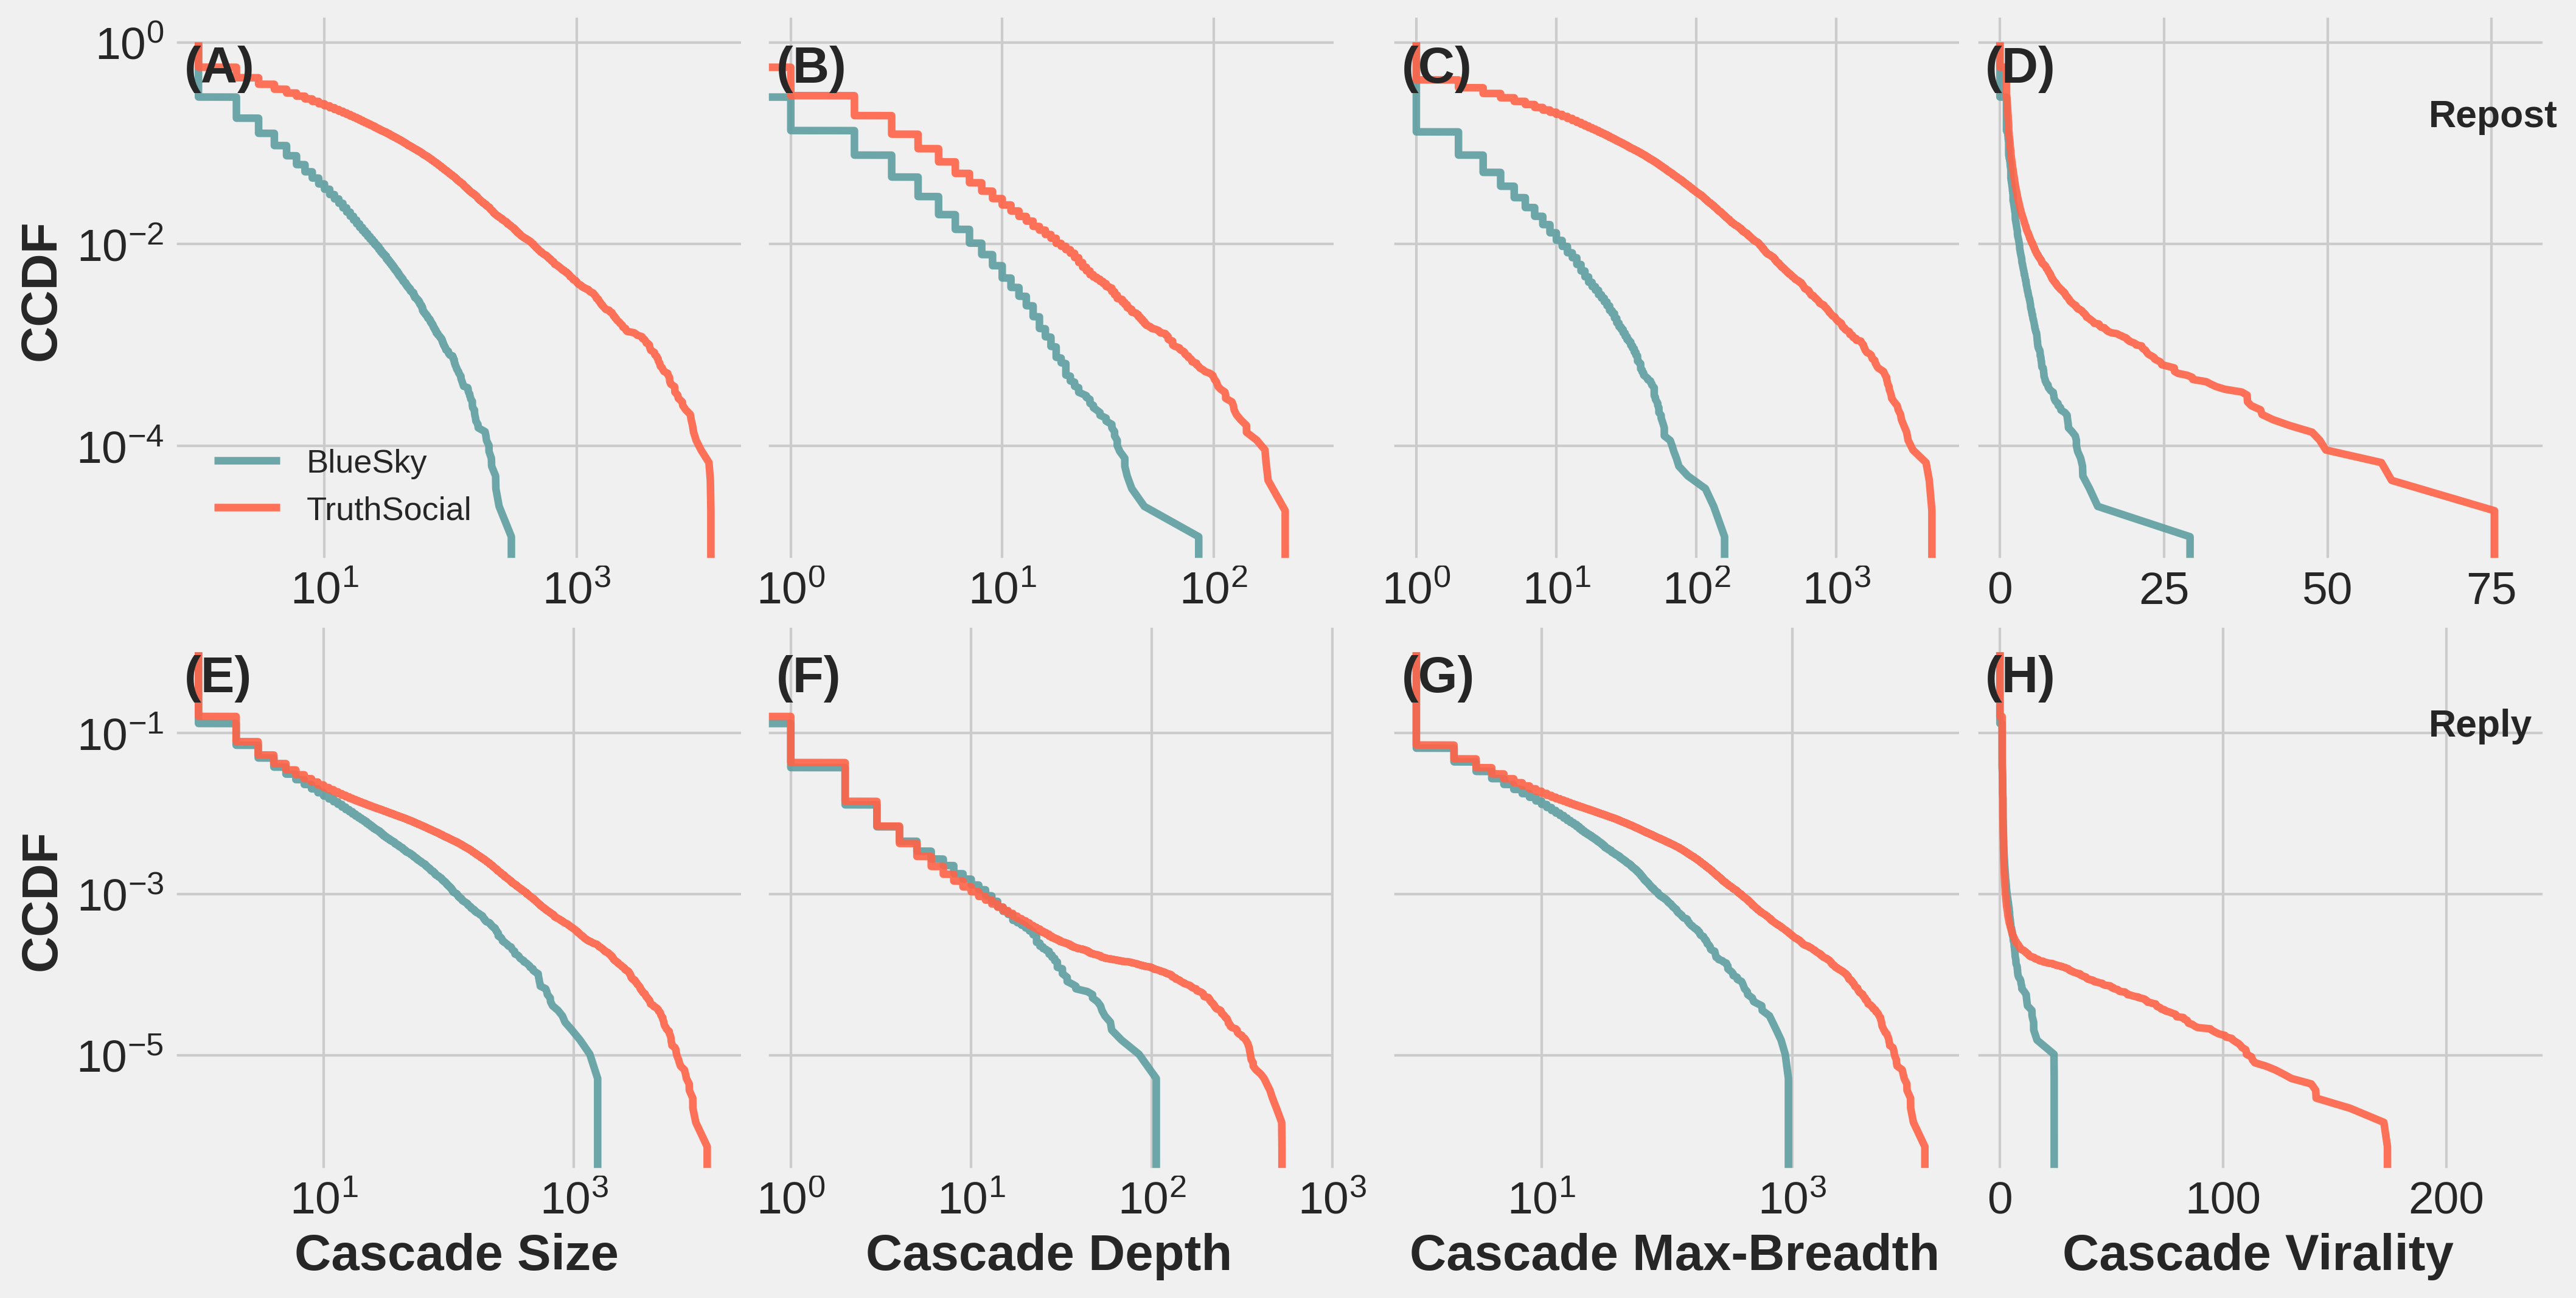
\includegraphics[width=\linewidth]{figures/ccdf_all.png}
\caption{(A--D) Complementary cumulative distribution functions (CCDFs) of repost cascade statistics across two platforms: BlueSky and TruthSocial. Each subplot represents a different structural property: Size, Depth, Breadth, and Structural Virality \cite{goel_structural_2016}. (E--H) The same analyses applied to reply cascades using the same metrics. X-axes are on a log scale (except for structural virality), and y-axes are on a log scale throughout. Each line represents a platform's empirical distribution.
}
\label{fig:ccdf}
\end{figure}

\begin{figure}[tb]
    \centering
    
\includegraphics[width=\linewidth]{figures/breadth_depth.png}
    \caption{(A--B) Robust Linear Models (RLM) regressions of log-transformed cascade breadth (A) and depth (B) on log-transformed cascade size for reply cascades on BlueSky and TruthSocial. (C--D) Same regressions for repost cascades. Point clouds represent individual cascades (semi-transparent), and lines represent RLM fits.}
    \label{fig:bd}
\end{figure}

As shown in Figure~\ref{fig:ccdf}, cascades on Truth Social appear larger, deeper, and broader than those on Bluesky for both reposts and replies, and show higher levels of structural virality. A straightforward explanation is platform size, since larger user bases mechanically allow cascades to expand further. Prior work has shown that depth, breadth, and structural virality all correlate positively with cascade size~\cite{juul_comparing_2021}, which raises a concern that marginal comparisons conflate structural effects with sheer volume. To address this, we hold cascade size constant and examine structural differences directly.

Figure~\ref{fig:bd} presents robust linear fits between log-transformed cascade size and both depth and breadth. After conditioning on cascade size, differences in repost behavior largely disappear: repost cascades scale similarly across Truth Social and Bluesky, with nearly identical slopes. In contrast, reply cascades exhibit a marked divergence. On Truth Social, replies tend to fan out, producing broad but shallow trees, whereas on Bluesky, conversations deepen through sequential exchange, forming narrower but more layered structures. This asymmetry suggests that while baseline amplification behaviors (reposts) are consistent, patterns of dialogic engagement diverge.

\subsection{Mechanisms of Structural Divergence}

\begin{table*}[]
\centering
\caption{Interaction Effects of Size (Log) and Platform on Breadth (Log) and Depth (Log)}
\label{model}
\begin{tabular}{lcccc}
\hline
\textbf{Model} & Size (Log) & Size (Log) $\times$ TruthSocial & $pseudo\ R^2$ & RMSE  \\
\hline
\hline
\multicolumn{5}{l}{\textbf{Breadth (Log)}} \\
\hline
Model 1 (Baseline) & $0.5043\ (0.0010)$ & $+0.4187\ (0.0012)$ & $0.9176$ & $0.1319$ \\
Model 2 (Influencers) & $0.5042\ (0.0010)$ & $+0.4121\ (0.0012)^{\dagger}$ & $0.9182$ & $0.1314$ \\
Model 3a (Composition) & $0.3692\ (0.0014)$ & $+0.2887\ (0.0019)$ & $0.9364$ & $0.1159$ \\
Model 3b (Alignment) & $0.1713\ (0.0012)$ & $+0.2362\ (0.0007)$ & $0.9432$ & $0.1095$ \\
Model 3c (Combined) & $0.2137\ (0.0016)$ & $+0.0706\ (0.0015)$ & $0.9546$ & $0.0979$ \\
Model 4 (Topic) & $0.5140\ (0.0014)$ & $+0.4260\ (0.0012)$ & $0.9191$ & $0.1307$ \\
\hline
\hline
\multicolumn{5}{l}{\textbf{Depth (Log)}} \\
\hline
Model 1 (Baseline) & $0.7320\ (0.0008)$ & $-0.3214\ (0.0009)$ & $0.8608$ & $0.1031$ \\
Model 2 (Influencers) & $0.7322\ (0.0008)$ & $-0.3134\ (0.0009)^{\dagger}$ & $0.8618$ & $0.1027$ \\
Model 3a (Composition) & $0.8432\ (0.0011)$ & $-0.1955\ (0.0015)$ & $0.8870$ & $0.0929$ \\
Model 3b (Alignment) & $0.9097\ (0.0010)$ & $-0.1889\ (0.0006)$ & $0.8926$ & $0.0905$ \\
Model 3c (Combined) & $0.9497\ (0.0014)$ & $-0.0491\ (0.0013)$ & $0.9085$ & $0.0835$ \\
Model 4 (Topic) & $0.7168\ (0.0011)$ & $-0.3302\ (0.0009)$ & $0.8623$ & $0.1025$ \\
\hline
\hline
\end{tabular}

\begin{minipage}{0.95\linewidth}
\footnotesize
\rev{\textit{Notes:} Robust linear models (Huber $M$-estimator) fitted with Huber's proposal 2 scale estimate; asymptotic standard errors in parentheses. Every coefficient shown is more than 25 standard errors from zero, so significance stars are omitted as uninformative. $N=123{,}189$ for every model.\\
\textsuperscript{†} Model 2 replaces the binary platform indicator with a three-category variable (Bluesky, Truth Social non-influencer, Truth Social influencer); the entry shown is the Truth Social non-influencer contrast against Bluesky.}
\end{minipage}
\end{table*}

The modeling results in Table~\ref{model} show clear differences in explanatory power across mechanisms. Model 2 (\textit{Influencers}) indicates that cascades initiated by high-follower accounts on Truth Social are only marginally broader, and the platform--size slope gap remains largely unchanged relative to baseline. The broad--shallow structure of Truth Social cascades thus reflects widespread interaction patterns across the platform, not merely the behavior of a small elite.

Model 3 (\textit{Ideological Structure}) is decomposed into three specifications. Composition alone (Model 3a) reduces divergence but leaves substantial residual differences \rev{($0.289$ for breadth, $-0.196$ for depth)}. In short, platform differences are not simply about the collective ideological leaning of users. Alignment alone (Model 3b) likewise attenuates but does not eliminate platform differences \rev{($0.236$ for breadth, $-0.189$ for depth)}. The combined model (3c) \rev{reduces both interaction terms by roughly five-sixths relative to the baseline, to $0.071$ for breadth and $-0.049$ for depth against baseline values of $0.419$ and $-0.321$}, showing that only when both ideological composition and cross-ideological alignment are considered together do platform-specific scaling gaps largely vanish. Model fit confirms this: pseudo-$R^2$ rises to \rev{$0.95$ for breadth and $0.91$ for depth} in Model 3c, with corresponding reductions in RMSE. \rev{The platform difference is therefore associated with both interaction alignment and broader differences in the ideological makeup of user communities, and neither covariate absorbs it alone.}

\rev{A limitation of this analysis is that the alignment ratio is computed from the same reply edges that determine cascade depth and breadth. Alignment and cascade structure are therefore jointly realized features of the same conversation, and their association does not establish a direction of influence. Cross-ideological exchanges may contribute to longer sequential discussions, but sustained conversations may also create conditions under which additional cross-ideological exchanges occur. Our analysis cannot distinguish between these processes. We therefore interpret ideological alignment as associated with cascade structure rather than as a causal determinant of it.}

Model 4 (\textit{Topic Variability}) shows \rev{no such effect. The platform-by-size interaction is essentially unchanged from the baseline once topic is included ($0.426$ against $0.419$ for breadth, $-0.330$ against $-0.321$ for depth), indicating that differences in what the two platforms discuss do not account for the difference in how their cascades grow.}

Taken together, the results clarify the hypotheses. H1 receives limited support: influencer status accounts for only a small share of the platform difference, indicating that Truth Social's broader and shallower reply cascades are not simply produced by high-follower users. H2 receives the strongest support: ideological composition and interaction alignment jointly eliminate most of the platform-specific divergence in scaling. H3 receives modest support: topic variability affects cascade geometry, but it explains far less of the platform difference than ideological structure. These results suggest that conversational diffusion is shaped less by who initiates cascades or what topic they discuss than by the ideological makeup of participants and the alignment of their interactions.


\subsection{Motif-Level Interaction Patterns}

\begin{figure*}[tb]
    \centering
    
\includegraphics[width=\linewidth]{figures/motif_z.png}
    \caption{\textbf{Chain motif analysis of cross-platform reply structures.}
    Standardized differences (Z-scores) in the frequency of three-node chain motifs between observed cascades and a randomized null model.
Node colors mark ideology (Left = blue, Center = green, Right = red); background shading groups motifs as aligned, mid-shift (middle node differs), end-shift (first or last node differs), or all-different.
Circles represent Truth Social, triangles Bluesky; gray symbols denote non-significant values ($|Z|<3$).}
    \label{fig:motif_zscore}
\end{figure*}

\paragraph{Chain motifs.}
We first examine chain motifs in reply cascades, which capture sequential exchanges where one reply receives another reply. Figure~\ref{fig:motif_zscore} shows how often three-node chain motifs occur relative to randomized reply-tree baselines. We organize these motifs into four ideological configurations: \textit{fully aligned} chains, in which all three users share the same ideological label; \textit{mid-shift} chains, in which the middle user differs ideologically from the first and final users; \textit{end-shift} chains, in which the final user differs from the first two users; and \textit{all-different} chains, in which all three users have different ideological labels. These configurations indicate whether sequential reply structures are built through ideologically aligned exchanges, cross-cutting interventions, or shifts in stance across conversational turns.

Fully aligned Center chains are consistently overrepresented on both platforms, indicating that center users often talk with one another. Fully aligned Right chains show no over- or under-representation on either platform, suggesting right-leaning users seldom sustain purely homogeneous conversations. Left-leaning chains diverge across platforms: Bluesky shows overrepresentation, whereas Truth Social shows underrepresentation.

The strongest contrasts appear in mid-shift ``bounce-back'' motifs. On Bluesky, all bounce-back chain motifs are overrepresented, indicating that cross-cutting replies across ideological pairings routinely draw responses. On Truth Social, only Left$\leftrightarrow$Right bounce-backs are overrepresented, but at much higher magnitudes than on Bluesky. This suggests that Bluesky exhibits a broader pattern of routine cross-cutting engagement, whereas on Truth Social, cross-cutting sequential exchange is concentrated in more intense confrontations between opposing ideological extremes.
%\cb{``truth social channels'' makes a strong agency claim about the platform encouraging these patterns but we dont know. You might simply say, on Truth Social, the pattern is prominently seen in intense confrontations between opposing extremes. Or something like that.  }

End-shift transitions (e.g., C--C--R, L--L--C) do not follow a uniform pattern. On Bluesky, end-shifts are generally at or below the rewired baseline, with L$\leftrightarrow$C links most underrepresented. On Truth Social, several center-involved end-shift motifs (R-C-C, R-R-L, L-C-C) are significantly overrepresented, suggesting that
%boundary exchanges among moderates or between moderates and rare left-leaning participants occur more often than expected by chance---
while the dominant bloc rarely incorporates cross-cutting voices, minority users (Center and Left) establish local footholds at the conversational boundary without full integration into mainstream exchanges.

\begin{figure*}
    \centering
    
\includegraphics[width=0.9\linewidth]{figures/star_motif_z.png}
    \caption{\textbf{Star motif analysis.} Standardized Z-scores of three-node star motif frequencies relative to degree-preserving null models.
Circles mark Truth Social, triangles Bluesky; gray symbols indicate non-significant values ($|Z|<3$).}
    \label{fig:star_motif}
\end{figure*}
%\cb{to be frank, i am not sure if i am getting a compelling story from the star analysis. i will attempt a simpler story rewrite, see what you think. you can also see a commented out concern with the original framing below (not visible in pdf but on latex)}
\paragraph{Star motifs.}
We next examine star motifs, which capture local branching in reply cascades: multiple users replying to the same parent post. Whereas chain motifs describe sequential extension across turns, star motifs describe how attention concentrates around a shared conversational object. Figure~\ref{fig:star_motif} summarizes standardized motif scores for three-node star motifs in reply cascades. Right-aligned (R–R–R) and center-aligned (C–C–C) stars are strongly overrepresented on Truth Social but suppressed on Bluesky, while left-aligned (L–L–L) stars show no significant over- or under-representation on either platform. This pattern suggests that homophilic clustering is not simply a majority-group phenomenon. Despite being the majority on Bluesky, left-leaning users do not cluster strongly in star formation.
Truth Social also shows overrepresentation of several mixed configurations (L--R--R, L--C--C, C--R--R, R--L--L). Most of these patterns correspond to a numerically rare ideology at the root, attracting a more dominant ideology pair as children. This is consistent with the minority voices (left-leaning users on Truth Social) drawing a disproportionate number of right-leaning response clusters. 

%on Truth Social fully aligned C--C--C and R--R--R stars are strongly overrepresented, while on Bluesky no comparable pattern appears. L--L--L stars are overrepresented on Bluesky but underrepresented on Truth Social. Truth Social also shows overrepresentation of several mixed configurations (L--R--R, L--C--C, C--R--R, R--L--L), indicating that diverse voices often cluster around a single root. These bursts of root-focused replies inflate breadth relative to depth: star motifs show Truth Social's tendency to channel heterogeneous engagement into short, centralized reply structures rather than sustained dialogue. \cb{not sure how this is showing that. we see a given motif is overrepresented but that doesnt really mean it is exactly replacing deep ones.}

%\cb{to be frank, i am getting a bit lost in these bits of info summarized and find it hard to see the connection between the regression and the motif work you are aiming to convince the reader of.}
\paragraph{Summary.}
The motif analysis shows that cross-ideological interaction is not a single structural process. On Truth Social, disagreement more often takes a branching form: multiple users respond to the same parent post, producing local breadth without sustained sequential exchange. On Bluesky, disagreement more often takes a chaining form: replies build on one another, producing depth through multi-turn interaction. Thus, the key difference is not whether ideological difference appears in conversations, but what shape it takes when it appears.



\section{Discussion}
This study compares how candidate-centered conversations about the 2024 U.S. presidential election unfold on two ideologically distinct but technically comparable platforms, Truth Social and Bluesky. Whereas most prior work emphasizes how far or how fast information spreads, we focus on structural form: whether interactions broaden outward through shallow branching or deepen through sequential layering. By analyzing both reposts and replies, we show that reposts scale similarly across platforms, but reply cascades diverge sharply: Truth Social supports broader, shallower exchanges, while Bluesky produces narrower, deeper threads. These results demonstrate that identical affordances can give rise to fundamentally different conversational dynamics, depending on the social and ideological composition of the communities that use them.

Our modeling results show that ideological composition and alignment together account for most of the platform divergence: cross-ideological exchanges are more likely to produce depth, while homogeneous cascades tend to flatten. Yet alignment alone is insufficient. Even when disagreement occurs, reply structures on Truth Social often remain shallow. 
Motif analysis clarifies this pattern: on Truth Social, disagreement frequently appears as star motifs---parallel replies directed at a single post. On Bluesky, disagreement more often takes the form of chain motifs, where replies build sequentially and support multi-turn interaction.

Motif results highlight the combined role of interactional structure and user composition. On Truth Social, left-leaning users constitute less than ten percent of the population, yet when present, they appear disproportionately in Left$\leftrightarrow$Right bounce-back motifs. This produces a paradox: such confrontational motifs are strongly overrepresented relative to the null model, but their absolute frequency is low, yielding the broad and shallow cascades seen in aggregate. Bounce-backs mark where cross-ideological debate occurs, but the scarcity of left-leaning users limits their influence on cascade structure. This also explains why alignment alone cannot account for platform differences: it captures whether interactions are within- or across-ideology, but not the underlying distribution of ideological groups.

These patterns also reveal a role for Center users that prior studies have largely overlooked. On Bluesky, they often appear as interlocutors in bounce-back motifs, serving as targets of cross-ideological replies and sustaining reciprocal exchanges. On Truth Social, they surface more frequently in end-shift motifs, acting as boundary bridges that connect minority voices without being integrated into dominant cascades. This contrast shows why centrist voices are simultaneously visible in local motifs yet remain marginal in aggregate cascade structures.

Although Truth Social and Bluesky provide similar affordances for posting, reposting, and replying, we do not interpret the observed differences as direct effects of platform design. The two platforms differ substantially in user base size, ideological composition, and patterns of interaction, and they may also differ in unobserved visibility and moderation processes. Our analysis therefore treats platform differences as emergent patterns in observed public interaction traces, rather than as causal effects of technical architecture.

These findings matter because they show that diffusion is not only about reach, speed, or volume, but also about the structure of participation. A cascade can become large through broad, shallow attention or through deeper sequential exchange, and these forms imply different kinds of political engagement. This distinction is especially important in a fragmented platform ecosystem, where newer platforms may share familiar Twitter-like affordances while supporting different conversational dynamics. By comparing reposts and replies separately, our study shows that amplification can scale similarly across platforms even when conversation diverges. Political diffusion should therefore be understood not only as whether information spreads, but as how participation is organized once it does.

Several limitations merit consideration. First, our analysis focuses on a single month during a politically salient period; whether these patterns hold across time and issues remains to be tested. Second, our measure of ideological alignment is coarse, relying on a simplified typology that may not capture subtler dimensions of identity. Third, while we account for cascade size, content, and user prominence, unobserved platform dynamics may shape interaction in ways we cannot fully disentangle. Finally, we use ``technical similarity'' in a deliberately narrow sense: both platforms provide Twitter-like affordances for posting, reposting, and threaded replying, which allows us to construct comparable cascade objects, though they differ in feed ranking, moderation, and recommendation architecture (see Appendix~\ref{app:platform_affordances}).

Nonetheless, by combining cascade-level modeling with motif analysis, this study advances a structural perspective on political diffusion. We focus not only on whether political conversations grow, but on how they scale: whether participation produces broad, shallow branching or deeper sequential exchange. This perspective allows us to compare which diffusion patterns appear stable across platforms and which are platform-specific. 

%Nonetheless, by combining cascade-level modeling with motif analysis, this study advances a structural perspective on political diffusion. \cb{To be frank, i think the claims of contributions below are not very easy to pinpoint and also a bit strawman-y. Other studies do not claim that it is platform design. I think you want to say that you focused on diffusion structure and scaling (which you already mention the the previous sentence), you performed cross-platform study to see which patterns are universal vs not, and for patterns that are different, you were able to identify a theoretically grounded mechanism that explains almost all of the differences observed. This is important because platforms come and go, we want to identify universal patterns of diffusion that can be applied to a new platform. Generally speaking, i would try to stay more literal in my discussion and implications, especially for this audience.} Rather than attributing outcomes to platform design alone, we describe emergent interaction patterns shaped by the communities and contexts in which they unfold. Understanding online political discourse thus requires not only tracing who speaks or what spreads, but also examining how conversational structures scaffold engagement itself.


\bibliography{aaai2026}

\section*{Paper Checklist}
\begin{enumerate}

\item For most authors...
\begin{enumerate}
    \item Would answering this research question advance science without violating social contracts, such as violating privacy norms, perpetuating unfair profiling, exacerbating the socio-economic divide, or implying disrespect to societies or cultures?
    
    \answerTODO{Yes.}

  \item Do your main claims in the abstract and introduction accurately reflect the paper's contributions and scope?
    
    \answerTODO{Yes.}

  \item Do you clarify how the proposed methodological approach is appropriate for the claims made?
    
    \answerTODO{Yes.}

  \item Do you clarify what are possible artifacts in the data used, given population-specific distributions?
    
    \answerTODO{Yes.}

  \item Did you describe the limitations of your work?
    
    \answerTODO{Yes.}

  \item Did you discuss any potential negative societal impacts of your work?
    
    \answerTODO{Yes.}

  \item Did you discuss any potential misuse of your work?
    
    \answerTODO{Yes.}

  \item Did you describe steps taken to prevent or mitigate potential negative outcomes of the research, such as data and model documentation, data anonymization, responsible release, access control, and the reproducibility of findings?
    
    \answerTODO{Yes.}

  \item Have you read the ethics review guidelines and ensured that your paper conforms to them?
    
    \answerTODO{Yes.}
\end{enumerate}

\item Additionally, if your study involves hypotheses testing...
\begin{enumerate}
  \item Did you clearly state the assumptions underlying all theoretical results?
    
    \answerTODO{Yes.}

  \item Have you provided justifications for all theoretical results?
    
    \answerTODO{Yes.}

  \item Did you discuss competing hypotheses or theories that might challenge or complement your theoretical results?
    
    \answerTODO{Yes.}

  \item Have you considered alternative mechanisms or explanations that might account for the same outcomes observed in your study?
    
    \answerTODO{Yes.}

  \item Did you address potential biases or limitations in your theoretical framework?
    
    \answerTODO{Yes.}

  \item Have you related your theoretical results to the existing literature in social science?
    
    \answerTODO{Yes.}

  \item Did you discuss the implications of your theoretical results for policy, practice, or further research in the social science domain?
    
    \answerTODO{Yes.}
\end{enumerate}

\item Additionally, if you are including theoretical proofs...
\begin{enumerate}
  \item Did you state the full set of assumptions of all theoretical results?
    
    \answerTODO{Not applicable.}

  \item Did you include complete proofs of all theoretical results?
    
    \answerTODO{Not applicable.}
\end{enumerate}

\item Additionally, if you ran machine learning experiments...
\begin{enumerate}
  \item Did you include the code, data, and instructions needed to reproduce the main experimental results (either in the supplemental material or as a URL)?
    
    \answerTODO{Yes, subject to platform terms and privacy constraints.}

  \item Did you specify all the training details (e.g., data splits, hyperparameters, how they were chosen)?
    
    \answerTODO{Not applicable. We use an existing instruction-tuned model and do not train a new model.}

  \item Did you report error bars (e.g., with respect to the random seed after running experiments multiple times)?
    
    \answerTODO{Not applicable for model training. We report uncertainty and robustness checks where relevant.}

  \item Did you include the total amount of compute and the type of resources used (e.g., type of GPUs, internal cluster, or cloud provider)?
    
    \answerTODO{Yes.}

  \item Do you justify how the proposed evaluation is sufficient and appropriate to the claims made?
    
    \answerTODO{Yes.}

  \item Do you discuss what is ``the cost'' of misclassification and fault (in)tolerance?
    
    \answerTODO{Yes.}
\end{enumerate}

\item Additionally, if you are using existing assets (e.g., code, data, models) or curating/releasing new assets, \textbf{without compromising anonymity}...
\begin{enumerate}
  \item If your work uses existing assets, did you cite the creators?
    
    \answerTODO{Yes.}

  \item Did you mention the license of the assets?
    
    \answerTODO{Yes, where applicable and available.}

  \item Did you include any new assets in the supplemental material or as a URL?
    
    \answerTODO{Yes, subject to platform terms and privacy constraints.}

  \item Did you discuss whether and how consent was obtained from people whose data you're using/curating?
    
    \answerTODO{Yes. The study uses publicly available social media data and does not involve direct interaction with users.}

  \item Did you discuss whether the data you are using/curating contains personally identifiable information or offensive content?
    
    \answerTODO{Yes.}

  \item If you are curating or releasing new datasets, did you discuss how you intend to make your datasets FAIR (see \citet{fair})?
    
    \answerTODO{Not applicable.}

  \item If you are curating or releasing new datasets, did you create a Datasheet for the Dataset (see \citet{gebru2021datasheets})?
    
    \answerTODO{Not applicable.}
\end{enumerate}

\item Additionally, if you used crowdsourcing or conducted research with human subjects, \textbf{without compromising anonymity}...
\begin{enumerate}
  \item Did you include the full text of instructions given to participants and screenshots?
    
    \answerTODO{Not applicable.}

  \item Did you describe any potential participant risks, with mentions of Institutional Review Board (IRB) approvals?
    
    \answerTODO{Not applicable.}

  \item Did you include the estimated hourly wage paid to participants and the total amount spent on participant compensation?
    
    \answerTODO{Not applicable.}

  \item Did you discuss how data is stored, shared, and deidentified?
    
    \answerTODO{Yes.}
\end{enumerate}

\end{enumerate}

%% -------------------------------------------------------
%% APPENDIX
%% -------------------------------------------------------
\appendix

\section{Power-Law Analysis of User-Level Activity Distributions}
\label{app:powerlaw}
We analyzed the distribution of user-level activity—specifically, the number of followers, reposts, and replies per user—across both platforms using power-law fits. Figure~\ref{fig:powerlaw} shows the complementary cumulative distribution functions (CCDFs) of these metrics in log-log scale, overlaid with fitted power-law tails (dashed orange lines). For each distribution, we report the estimated power-law exponent $\gamma$ and the lower cutoff $x_{\min}$ above which the power-law holds.

The distribution of follower counts reveals strong skewness on both platforms. On Truth Social, a small number of users amass an exceptionally large following, with $\gamma = 1.76$ and $x_{\min} \approx 13{,}515$. Bluesky shows a slightly less extreme concentration ($\gamma = 1.84$, $x_{\min} \approx 1{,}498$). Repost and reply behaviors also exhibit heavy-tailed patterns. On Bluesky, replies decay rapidly ($\gamma = 3.02$) while reposts follow a shallower slope ($\gamma = 2.43$). Truth Social displays flatter distributions for both reposts ($\gamma = 1.84$) and replies ($\gamma = 1.79$), consistent with broader participation from users in redistributing and responding to content.

\subsection*{Exclusion of Highly Followed Users for Robustness.}
To identify unusually influential users, we examined the follower-count distribution on each platform. On Truth Social, we observed a marked discontinuity in the upper tail: a gap in the follower-rank plot revealed a distinct separation between the top 8 users and the rest of the distribution. Based on this natural break, we designated these 8 users as outliers for modeling purposes. This data-driven threshold captures extreme influence without imposing arbitrary cutoffs.

\begin{figure}
    \centering
    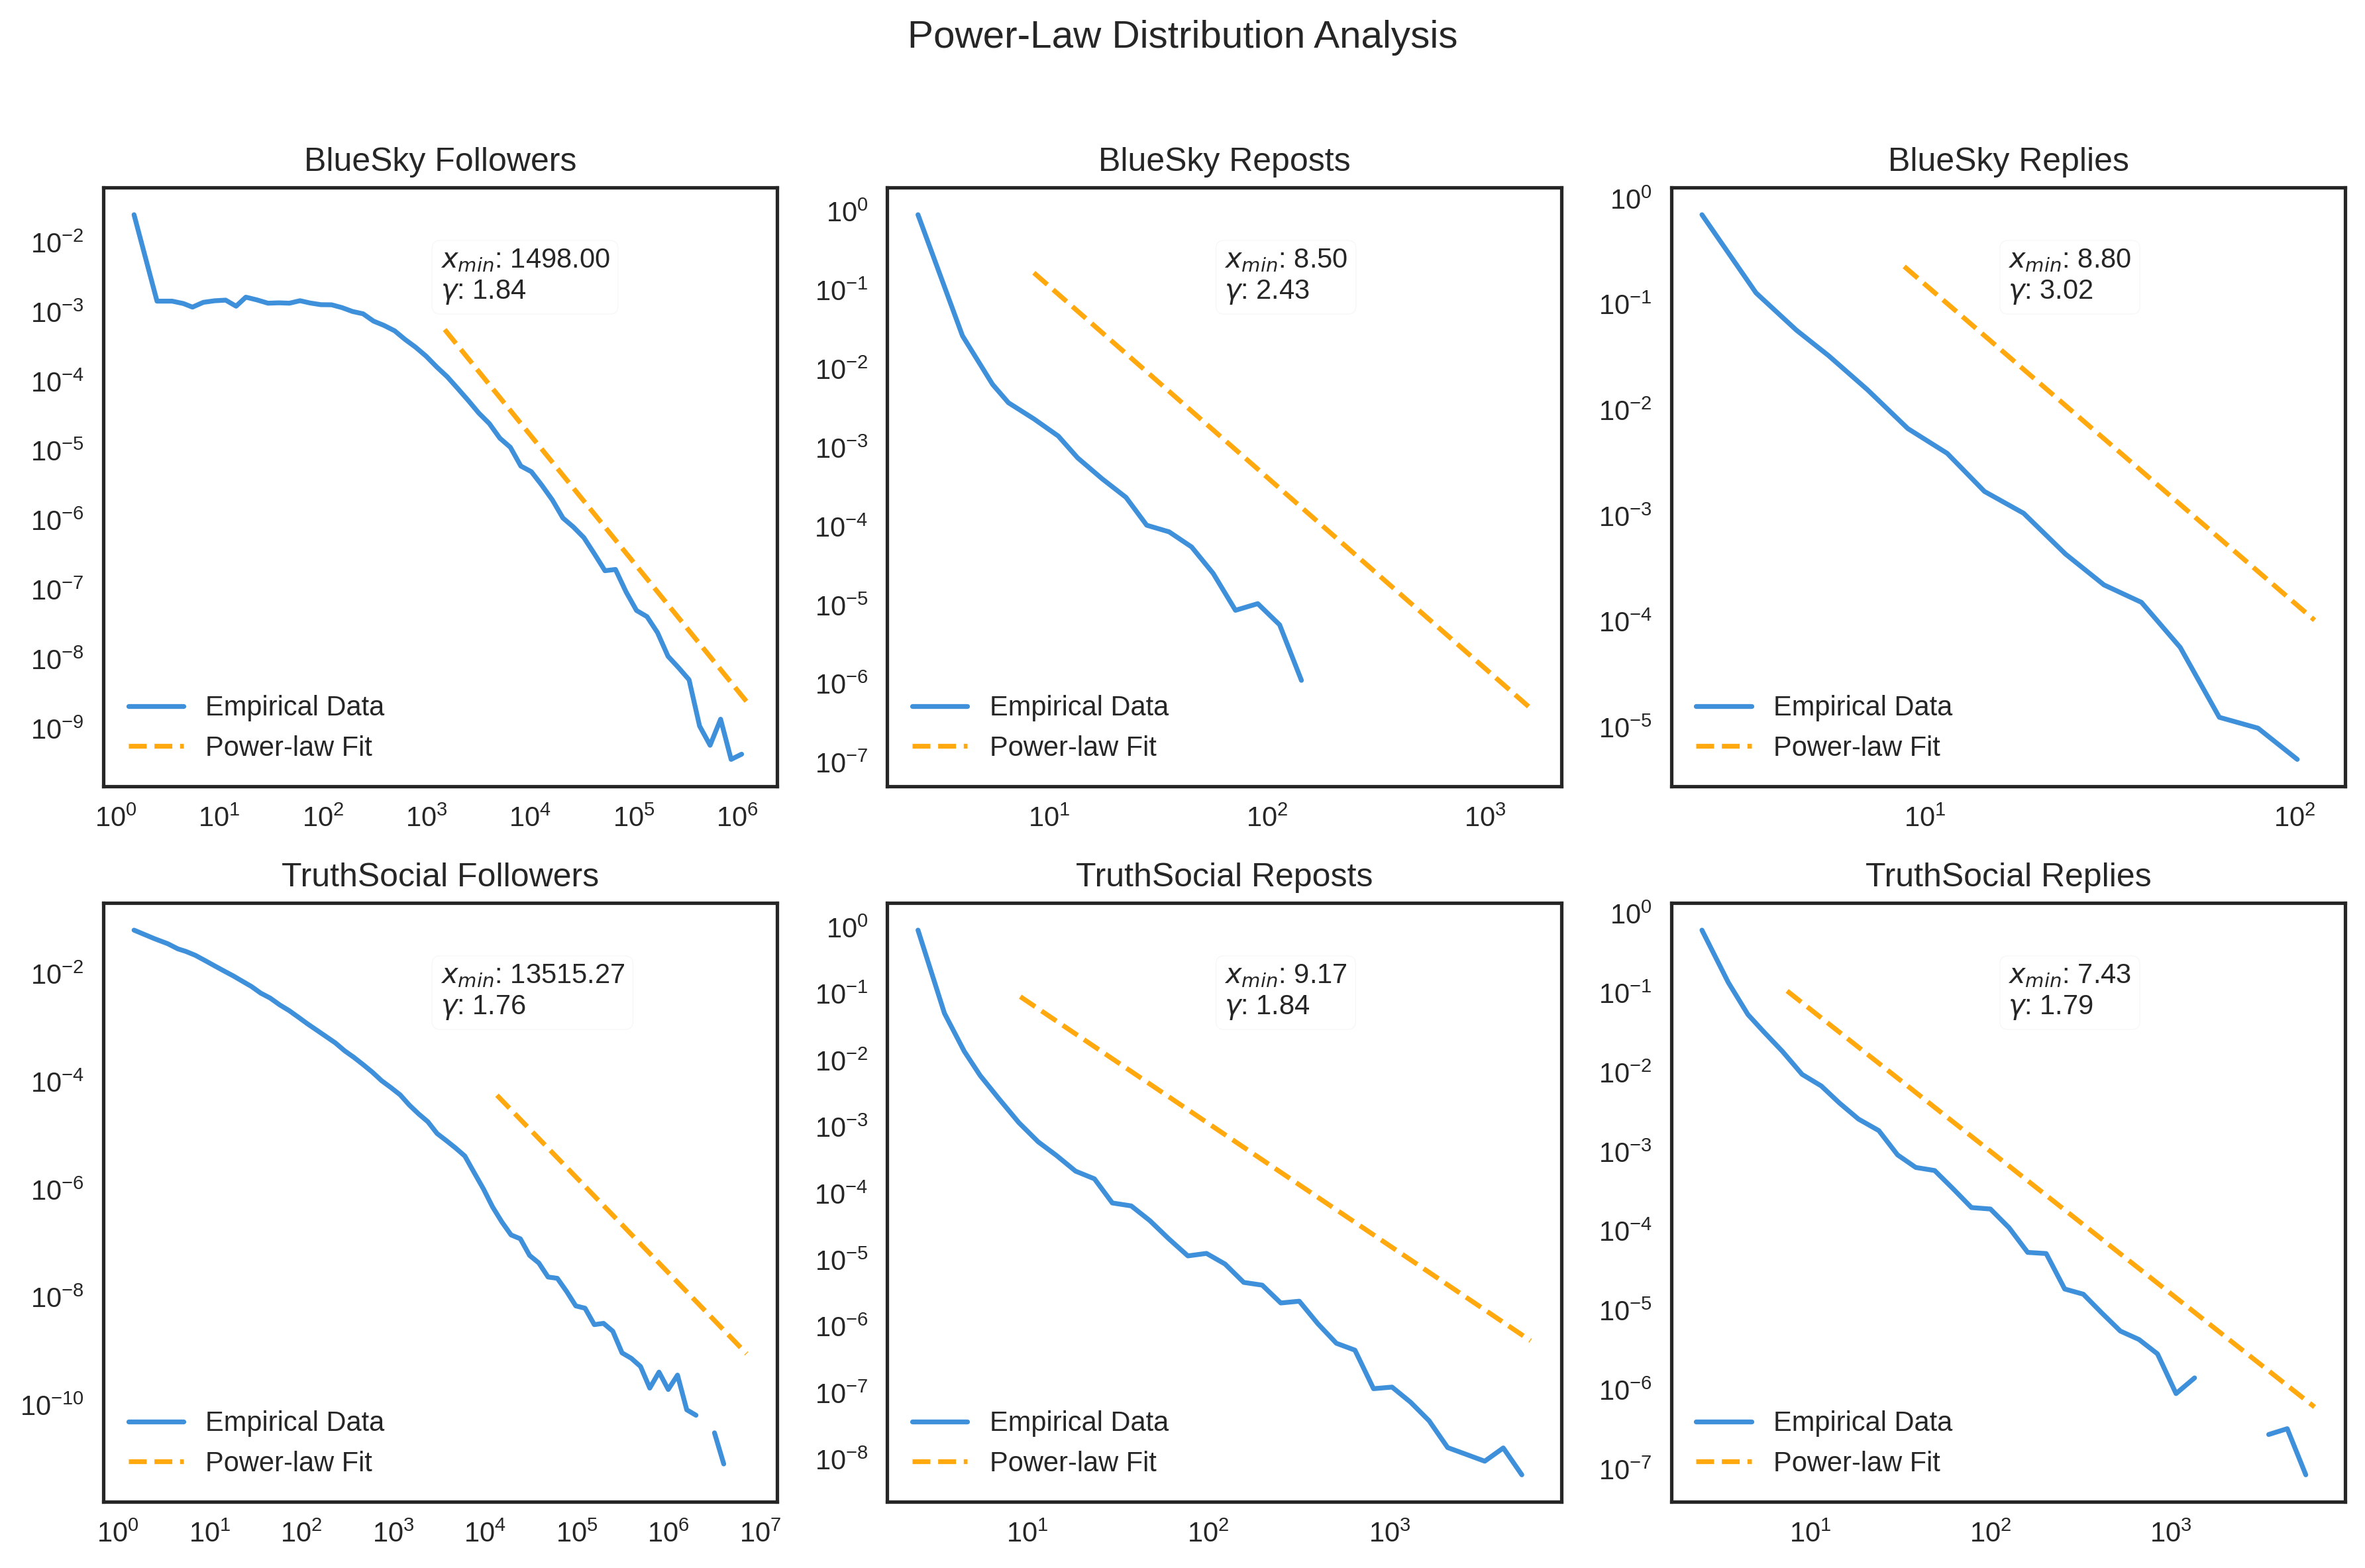
\includegraphics[width=\linewidth]{figures/powerlaw.png}
    \caption{Follower count distributions across platforms.}
    \label{fig:powerlaw}
\end{figure}

\section{Ideology Estimation: Validation and Robustness}
\label{app:ideology_distribution}
\subsection*{Ideological Distribution of Root Post Authors.}
Figure~\ref{fig:party_dis} shows the ideological distribution of users who authored root posts. Bluesky exhibited a predominantly left-leaning user base (over 46,000 root posts from left-leaning users vs.\ 27,495 from right-leaning), while Truth Social was overwhelmingly right-leaning (37,639 right-authored root posts vs.\ 5,149 from left-leaning users and 1,053 from centrists).

\begin{figure*}
    \centering
    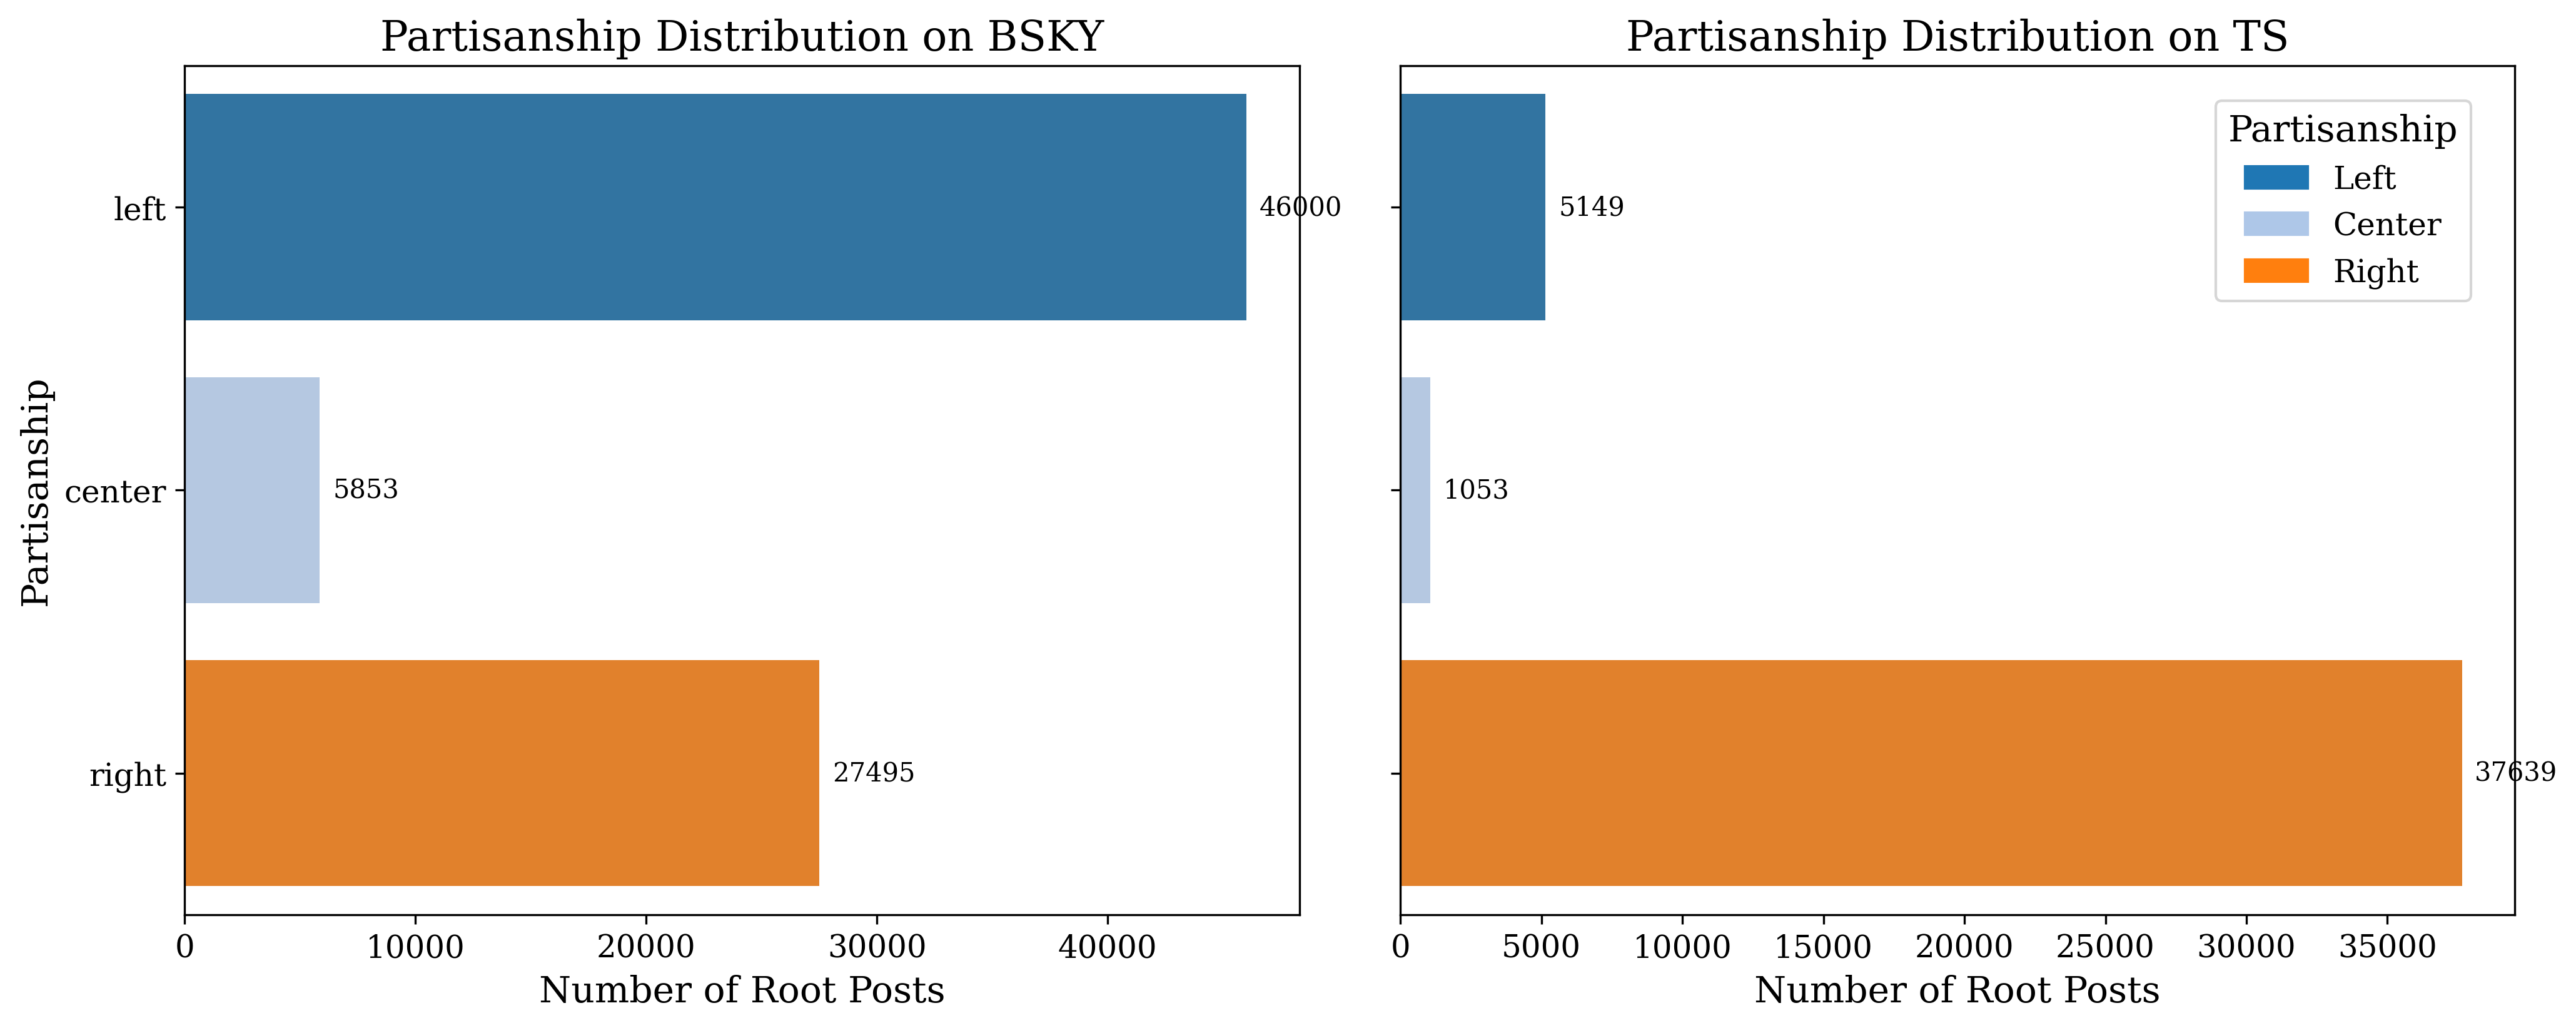
\includegraphics[width=\linewidth]{figures/party_dis.png}
    \caption{Distribution of root post partisanship across platforms.
Bar plots show the number of root posts authored by users with left-leaning, centrist, or right-leaning stance labels. On \textit{Bluesky}, left-leaning users dominate root-post activity. \textit{Truth Social} exhibits a pronounced right-leaning skew. These distributions reflect the ideological clustering of user bases on each platform.}
    \label{fig:party_dis}
\end{figure*}

\subsection*{Robustness to Ideology Thresholds.}
We re-estimated Model~3 using alternative thresholds of 0.5 and 0.7 for classifying user ideology. As shown in Table~\ref{tab:robust_threshold} and Figure~\ref{fig:threshold}, the results remain substantively consistent across thresholds: pseudo-$R^2$ values are uniformly high, error metrics fluctuate only marginally, and the platform--size interaction decreases markedly once ideological structure is incorporated at all thresholds. We also applied an unsupervised natural breakpoint detection algorithm to the ideology distribution, which identified 0.67 as a statistically distinct split point; we adopt 0.6 as our default to avoid excessive sparsity.

\begin{figure*}
    \centering
    
\includegraphics[width=0.9\linewidth]{figures/threshold.png}
    \caption{User ideology proportions and consistency across thresholds on \textit{Bluesky} and \textit{Truth Social}. Left-leaning users dominate at lower thresholds on Bluesky; right-leaning users represent the majority on Truth Social at all thresholds. Center-labeled users increase at higher thresholds on both platforms.}
    \label{fig:threshold}
\end{figure*}

\begin{table*}[htbp]
\centering
\caption{Robustness check using alternative thresholds for defining user-level ideology.
Results show that the main findings are stable across thresholds (0.5, 0.6, 0.7):
platform gaps in cascade breadth and depth are consistently reduced once ideological structure is accounted for.}
\label{tab:robust_threshold}
\begin{tabular}{ccccc|cccc}
\hline
 & \multicolumn{4}{c}{Breadth (Log)} & \multicolumn{4}{c}{Depth (Log)} \\
\hline
 Threshold& Pseudo-$R^2$ & MAE & RMSE & Size$\times$TS  & Pseudo-$R^2$ & MAE & RMSE & Size$\times$TS  \\
\hline
0.5 & 0.948 & 0.041 & 0.104 & 0.127 &  0.901 & 0.036 & 0.087 & -0.143  \\
0.6 & 0.952 & 0.042 & 0.101 & 0.023 & 0.905 & 0.036 & 0.085 & -0.050  \\
0.7 & 0.955 & 0.041 & 0.097 & 0.000 &  0.911 & 0.035 & 0.083 & -0.000  \\
\hline
\end{tabular}
\end{table*}

% \section{Topic Distribution}
% \label{app:topicdis}
% To compare topical emphasis across platforms, we plotted the distribution of root posts by topic label for \textit{Bluesky} and \textit{Truth Social} (Fig.~\ref{fig:topic_dis}). While both platforms exhibited substantial engagement with topics surrounding Donald Trump’s legal issues and the 2024 U.S. presidential election, there were notable differences. Posts on \textit{Bluesky} were more likely to focus on legal accountability, international affairs (e.g., the Israel–Hamas conflict), and broader campaign discourse. In contrast, \textit{Truth Social} featured a larger proportion of posts celebrating Trump (e.g., birthdays and tributes) and promoting pro-Trump narratives (e.g., “MAGA advocacy”), reflecting differences in user base ideology and agenda-setting priorities. These topical variations underscore the divergent discourse ecosystems that have emerged across platforms.


\section{Modeling Strategy and Regression Diagnostics}
\label{app:strategy}
Initial Ordinary Least Squares (OLS) regression revealed strong heteroskedasticity, with residuals showing a fan-shaped pattern as a function of fitted values (Figure~\ref{fig:model_diag}). Residuals also exhibited heavy tails resembling a t-distribution. Although Cook's Distance analysis identified a small number of observations with relatively higher influence, the vast majority fell well below the threshold of $4/n$. \rev{The heavy-tailed, heteroskedastic residuals motivate robust estimation, and all models reported in the main text are robust linear models with the Huber loss. Because 61.3\% of reply cascades consist of a root post with no replies, and these sit exactly at the origin of the log--log scaling plot, the default median-absolute-deviation scale estimate collapses toward zero; standard errors computed from it are not interpretable. We therefore fit with Huber's proposal 2 scale, which does not degenerate here, and report a sensitivity analysis across samples and scale estimators below. The one analysis estimated by OLS with HC3 errors is the repost reconstruction robustness check, where lattice-valued outcomes make the Huber scale estimate degenerate.}

\begin{figure*}
    \centering
    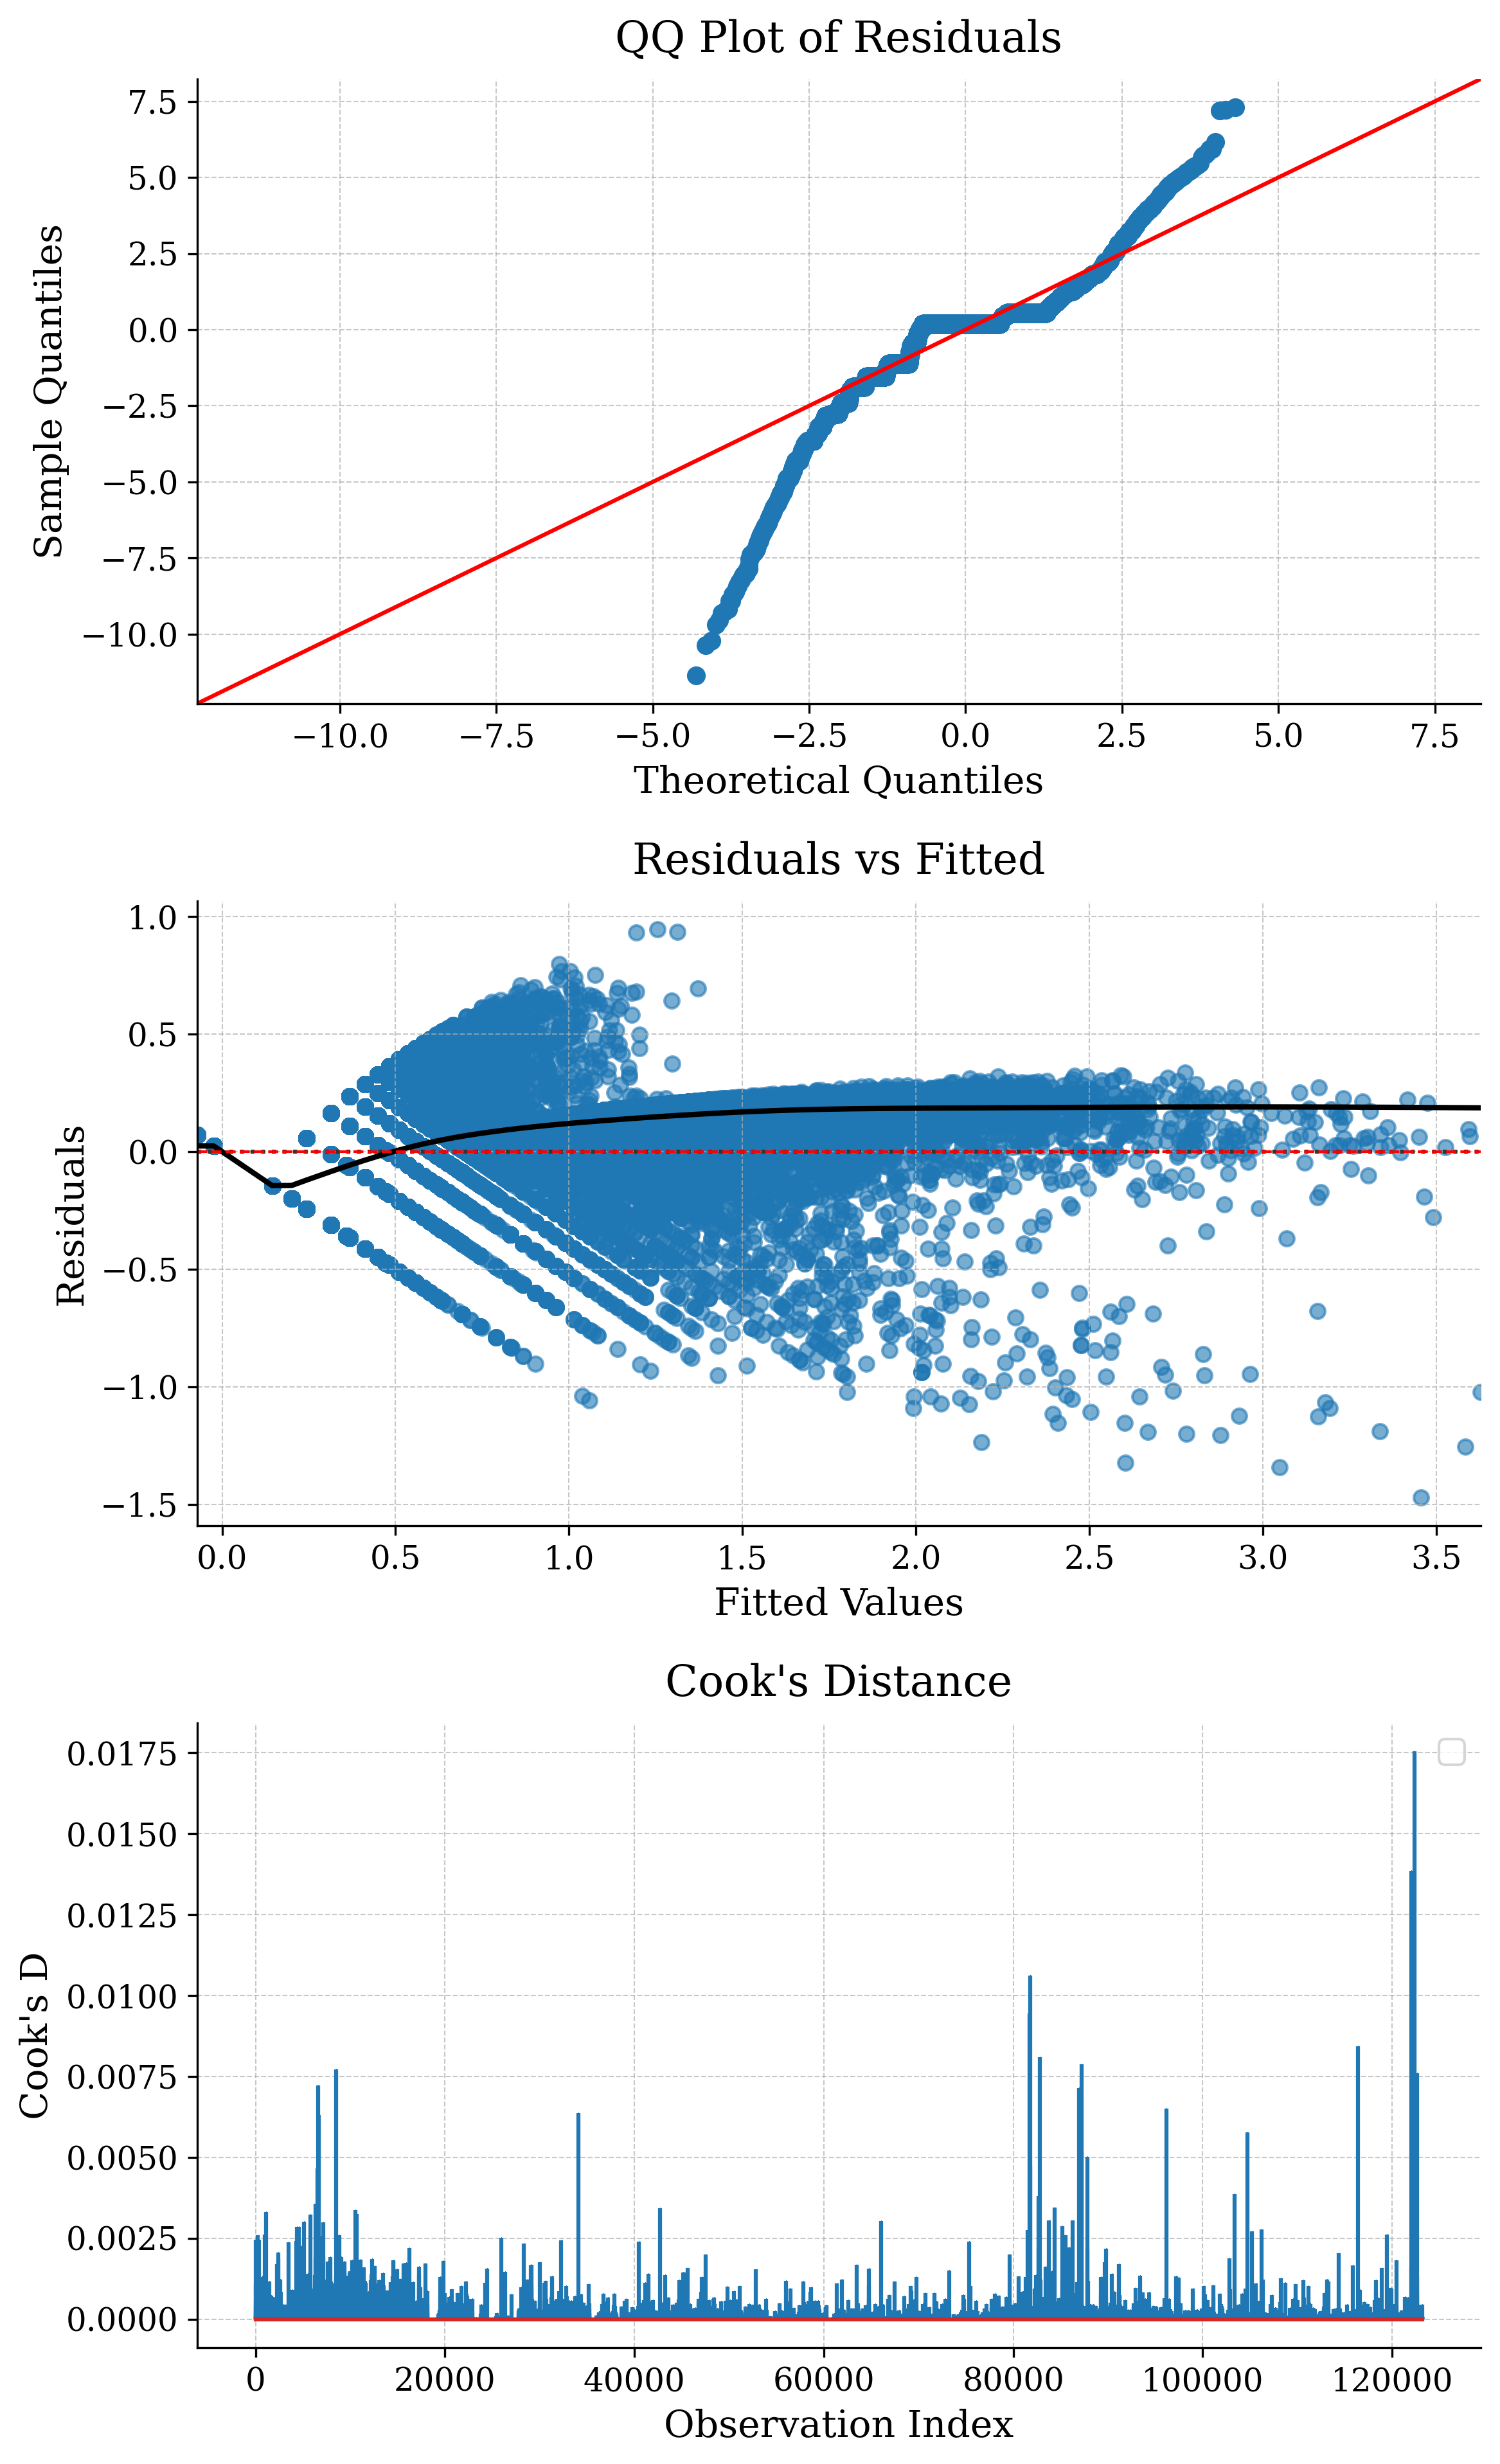
\includegraphics[width=0.7\linewidth]{figures/model_diag.png}
    \caption{\textbf{Regression diagnostic plots.}
Top: quantile--quantile (QQ) plot of residuals indicating heavy-tailed error distribution. Bottom: residuals vs.\ fitted values showing a fan-shaped pattern (heteroskedasticity). LOESS smoother overlaid.}
    \label{fig:model_diag}
\end{figure*}

\section{Spline Transformations}
\label{app:spline}
To examine potential nonlinear predictor effects, we inspected partial residual plots for \texttt{author\_left\_ratio}, \texttt{author\_right\_ratio}, and \texttt{author\_alignment\_ratio} (Figure~\ref{fig:partial_residuals}). \texttt{author\_left\_ratio} shows a convex pattern (residuals above zero at both ends), motivating a spline basis. \texttt{author\_alignment\_ratio} shows a monotonic but curved relationship with increasing slope near 1, also motivating a spline. \texttt{author\_right\_ratio} appears approximately linear and is retained as a simple linear term. We apply spline transformations (\texttt{bs} basis, df\,=\,3) to \texttt{author\_left\_ratio} and \texttt{author\_alignment\_ratio}; B-splines are preferred over natural cubic splines here because the data are confined to [0,1] and used in interactions, where their local support provides greater numerical stability.

\begin{figure*}
\centering
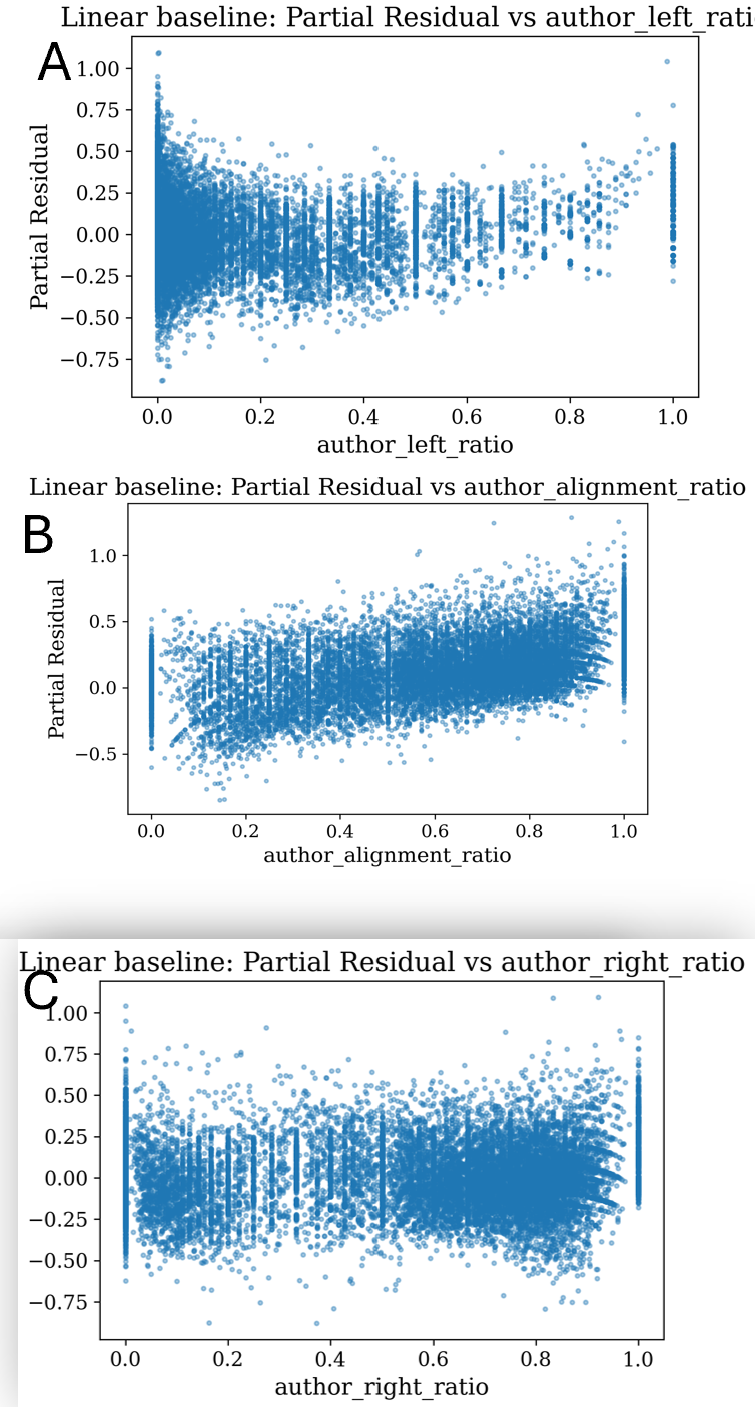
\includegraphics[width=0.6\linewidth]{figures/partial.png}
    \caption{Partial residual plots under a linear baseline for (A) \texttt{author\_left\_ratio}, (B) \texttt{author\_right\_ratio}, and (C) \texttt{author\_alignment\_ratio}.}
    \label{fig:partial_residuals}
\end{figure*}

\section{Final Model Specification}

Our final model specification includes: (1) a main effect of \texttt{log\_size} and its interaction with \texttt{platform}; (2) \texttt{right\_user\_ratio} and spline-based transformations of \texttt{alignment\_ratio} and \texttt{left\_user\_ratio}, interacted with both \texttt{log\_size} and \texttt{platform}; and (3) topic category and outlier status as categorical moderators. All models were estimated using the \texttt{statsmodels} package in Python with robust standard errors.

\section{Robustness Checks: Alternative User Composition Specifications}
\label{app:robustcheck}
To assess whether findings depend on how user composition is encoded, we compared four specifications: (1) left/right shares only, (2) majority/minority shares only, (3) left/right with alignment, and (4) majority/minority with alignment. Table~\ref{tab:si_comp_encoding_rlm_full} reports results for both cascade breadth and depth.

Including alignment substantially improves fit for both outcomes (Breadth $R^2 \approx 0.95$; Depth $R^2 \approx 0.90$), confirming that interaction structure plays a central role in cascade geometry. The majority/minority framework slightly improves error metrics and consistently reduces the size of the $\log(\text{size}) \times \text{platform}$ interaction, but the overall improvement relative to left/right is modest. We retain the left/right specification as our main model for theoretical interpretability.

\begin{table*}[t]
\centering
\caption{Comparison of user-composition encodings (Left/Right vs. Majority/Minority), with and without alignment. Robust Linear Models.}
\label{tab:si_comp_encoding_rlm_full}
\scriptsize
\renewcommand{\arraystretch}{1.25}
\setlength{\tabcolsep}{3pt}

\begin{tabular}{lcccccccc}
\hline
& \multicolumn{4}{c}{\textbf{Panel A: Composition only}} & \multicolumn{4}{c}{\textbf{Panel B: + Alignment (df=3)}}\\
\cline{2-9}
& \multicolumn{2}{c}{\textbf{Breadth (log\_breadth)}} & \multicolumn{2}{c}{\textbf{Depth (log\_depth)}} & \multicolumn{2}{c}{\textbf{Breadth (log\_breadth)}} & \multicolumn{2}{c}{\textbf{Depth (log\_depth)}}\\
\cline{2-9}
& L/R & Maj/Min & L/R & Maj/Min & L/R+Align & Maj/Min+Align & L/R+Align & Maj/Min+Align \\
\hline
Observations & 123{,}189 & 123{,}189 & 123{,}189 & 123{,}189 & 123{,}189 & 123{,}189 & 123{,}189 & 123{,}189 \\
Pseudo $R^{2}$ & 0.9312 & \textbf{0.9322} & \textbf{0.8781} & 0.8767 & \textbf{0.9517} & 0.9508 & \textbf{0.9049} & 0.9041 \\
MAE & 0.0565 & \textbf{0.0563} & 0.0445 & \textbf{0.0431} & \textbf{0.0427} & 0.0411 & 0.0368 & \textbf{0.0359} \\
RMSE & 0.1205 & \textbf{0.1196} & \textbf{0.0964} & 0.0970 & \textbf{0.1010} & 0.1019 & \textbf{0.0852} & 0.0855 \\
\\
$\beta_{\log(\text{size})}$
& 0.3646 & 0.3562 & 0.9002 & 0.8982 & 0.2526 & 0.4807 & 0.9286 & 0.8023 \\
$\beta_{\log(\text{size})\times \text{platform(ts)}}$
& $0.2579$ & $0.1073$ & $-0.1950$ & $-0.1112$ & $0.0230$ & $0.0719$ & $-0.0547$ & $-0.0552$ \\
\hline
\end{tabular}

\vspace{0.75ex}
\footnotesize
\textit{Notes:}
L/R models the \emph{left-user share} with a spline (df=3) and the \emph{right-user share} linearly, interacted with $\log(\text{size})$ and platform.
Maj/Min re-codes composition by platform-dominant ideology (majority) vs.\ opposing (minority); majority share modeled with a spline (df=3), minority share linearly.
Panel~B additionally includes the \emph{alignment ratio} (spline, df=3) and its interactions.
\end{table*}

\section{Marginal Effects of Ideological Structure}

Figure~\ref{fig:marginal} plots marginal effects of alignment ratio, left-user ratio, and right-user ratio on cascade structure. For \textbf{depth}, higher alignment is associated with shallower structures, consistent with the idea that ideologically homogeneous cascades sustain fewer extended exchanges. Cascades with fewer right-leaning participants exhibit greater layering, echoing the motif finding that right-leaning users rarely construct fully right-aligned chains. The marginal effects of left- and right-user ratios are asymmetric: increases in right-leaning participation are linked to sharper declines in depth than comparable increases in left-leaning participation. For \textbf{breadth}, higher alignment corresponds to wider cascades, indicating that homogeneous groups are more likely to generate simultaneous uptake at the same level. The left-user ratio exhibits an inverted-U relationship with breadth, while the right-user ratio shows a more linear pattern: as right-leaning users become increasingly dominant, cascades grow consistently broader.

\begin{figure*}
    \centering
    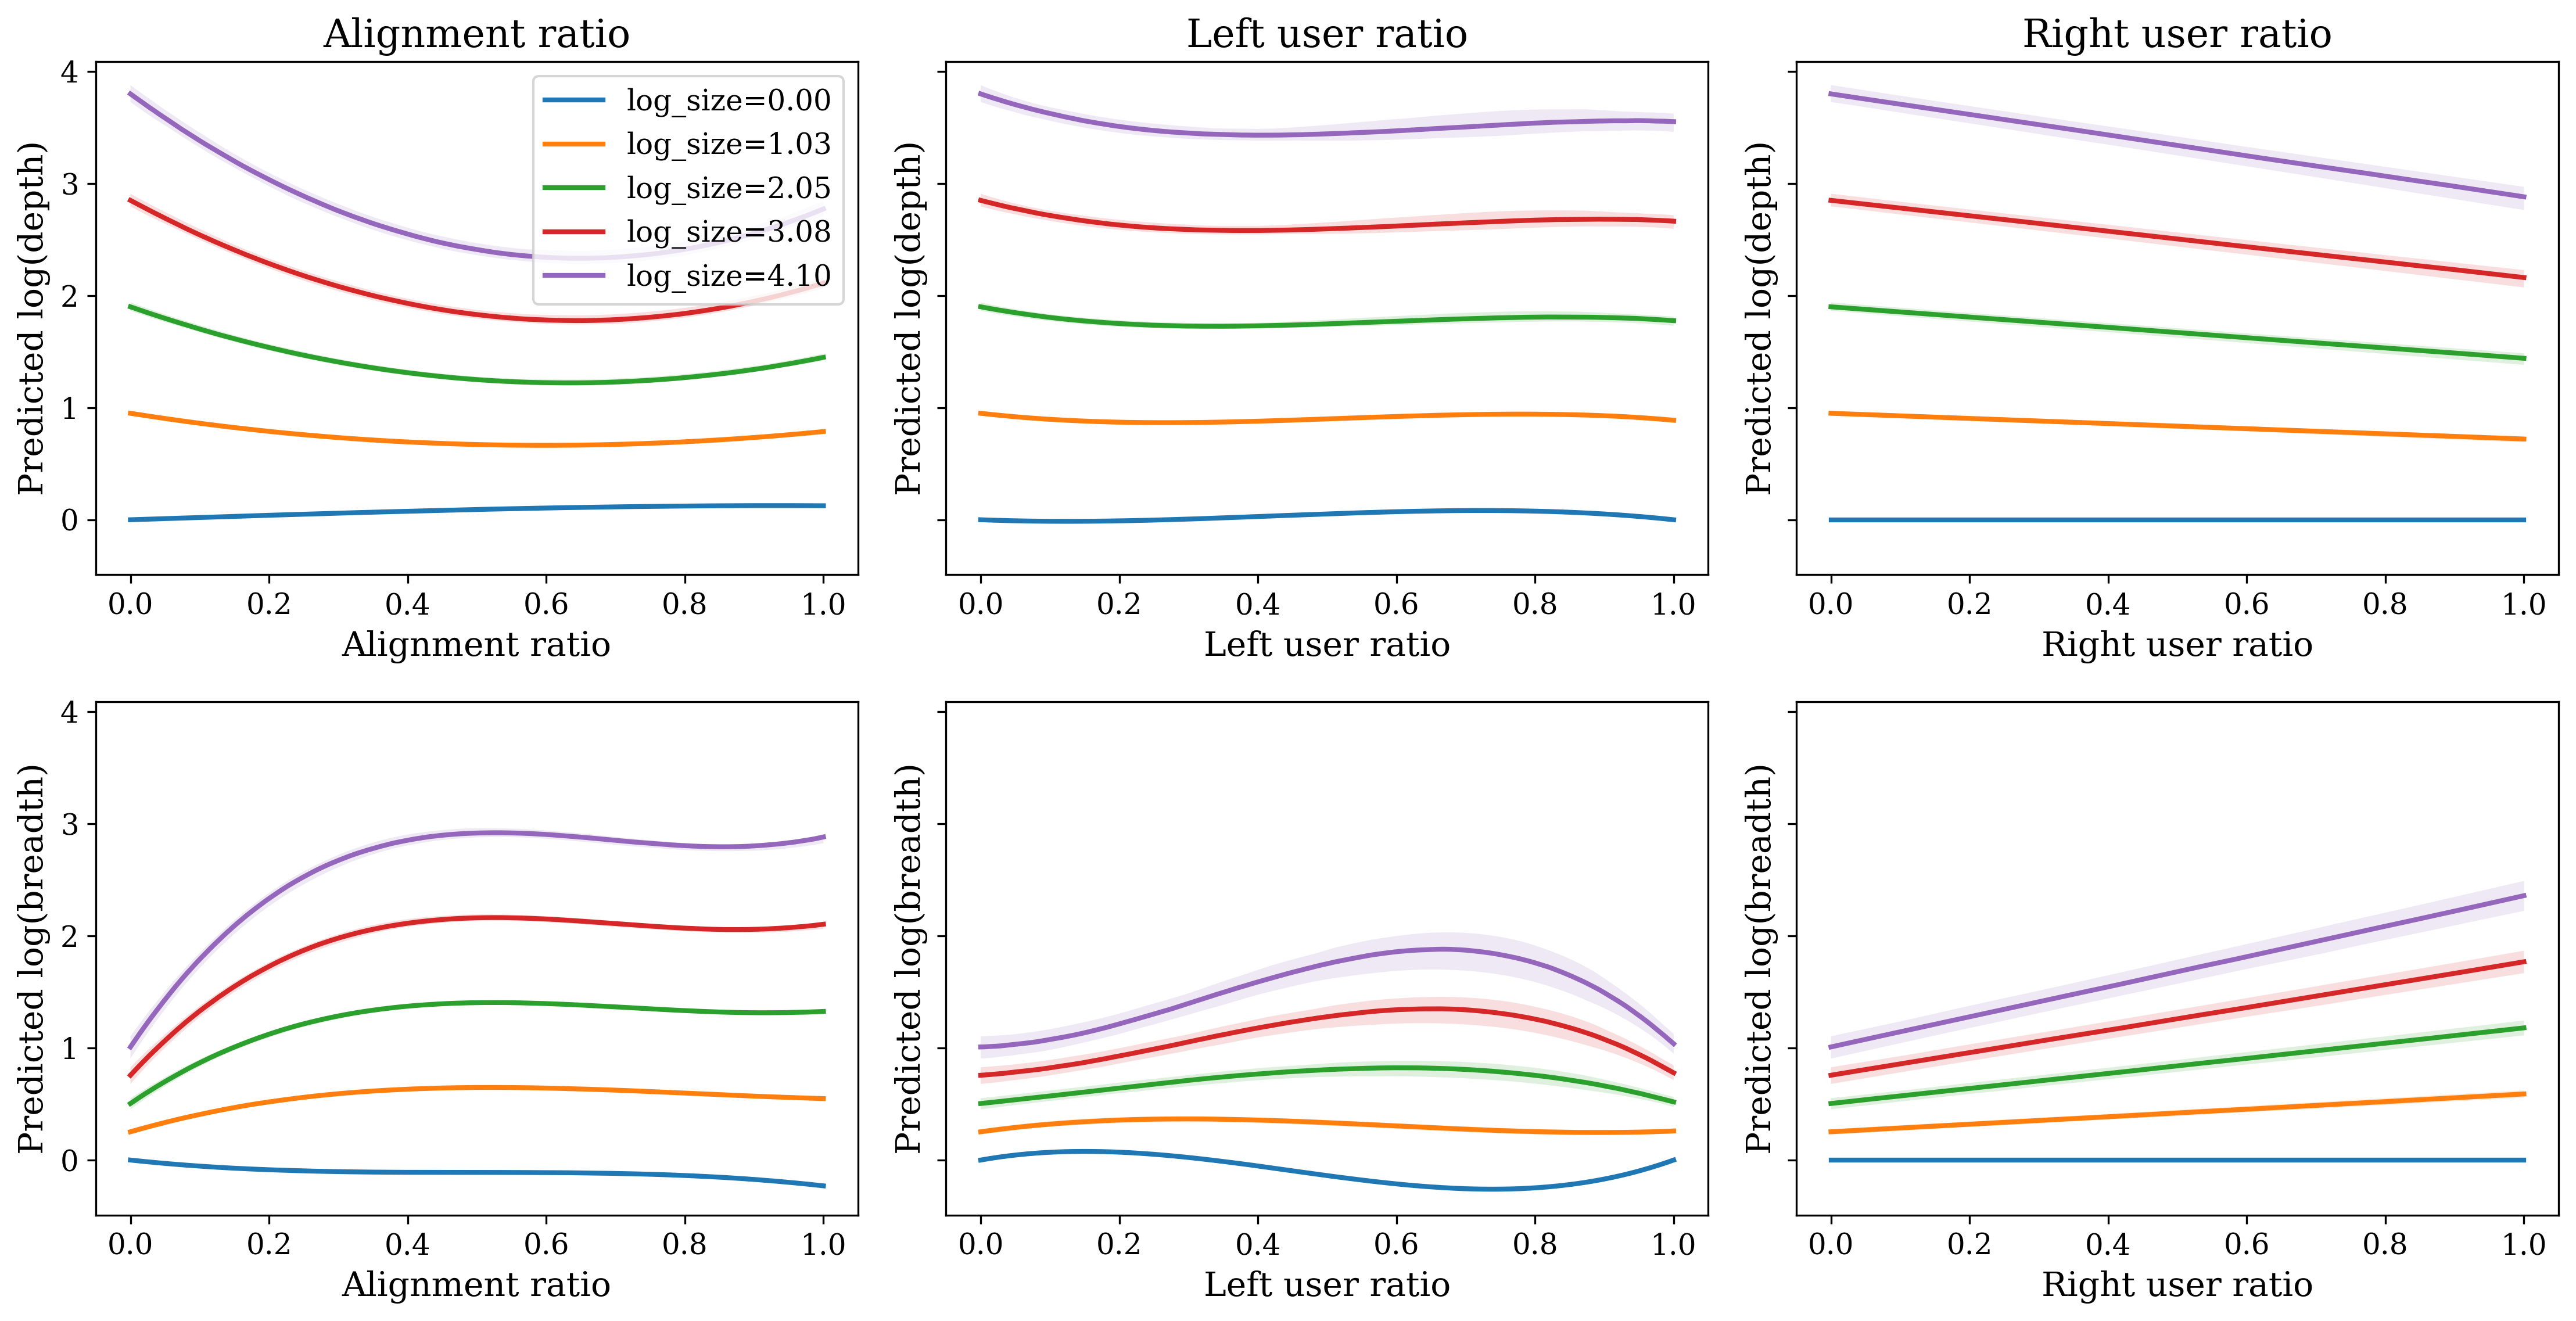
\includegraphics[width=\linewidth]{figures/model_margin_effect.png}
    \caption{Marginal effects of ideological alignment, left-user ratio, and right-user ratio on cascade structure.
Solid lines denote predicted log(depth) (top row) and log(breadth) (bottom row) at five equally spaced values of log(size). Shaded bands represent 95\% bootstrap confidence intervals. Homogeneous cascades (high alignment) tend to flatten into wide, shallow structures; heterogeneous cascades deepen through sequential exchanges.}
    \label{fig:marginal}
\end{figure*}


\section{Platform Affordances and Technical Comparability}
\label{app:platform_affordances}

Our comparison rests on a narrow notion of technical comparability: we do not assume the platforms are identical exposure environments, but that they share Twitter-like affordances (posting, reposting, threaded replies) that enable construction of comparable cascade objects. Ranking systems, moderation decisions, and feed settings may affect which posts users see and which cascades grow; these are partly opaque and cannot be fully identified from public traces. Our analysis should be interpreted as an observational comparison of public interaction traces, not a causal estimate of platform design effects.

The technical lineage of both platforms provides additional justification. Bluesky is built on the AT Protocol, which also supports custom feed generation through a feed-generator architecture. Truth Social has been widely documented as Mastodon-derived, using open-source social networking software with visual modifications. These lineages support structural comparability of cascade objects while reinforcing that ranking, moderation, and exposure should be treated as platform-specific and only partially observed.

\begin{table}[ht]
\centering
\small
\caption{Platform affordances and technical lineage relevant to cascade construction.}
\label{tab:platform_affordances}
\begin{tabular}{p{0.23\linewidth}p{0.32\linewidth}p{0.32\linewidth}}
\toprule
\textbf{Dimension} & \textbf{Truth Social} & \textbf{Bluesky} \\
\midrule
Technical lineage
& Mastodon-derived platform
& Built on the open-source AT Protocol ecosystem \\

Posting affordance
& Supports user-authored posts
& Supports user-authored posts \\

Reposting affordance
& Supports repost-style resharing
& Supports repost-style resharing \\

Reply affordance
& Supports threaded replies
& Supports threaded replies \\

Cascade observability
& Public repost and reply traces observable
& Public repost and reply traces observable \\

Feed and ranking
& Platform-specific visibility and ranking; not directly observed
& Multiple feeds via feed-generator architecture; visibility varies \\

Moderation
& Platform-specific moderation may affect observed patterns
& Decentralized moderation and curation may affect patterns \\

Analytic implication
& Enables cascade construction; exposure process not fully identified
& Enables cascade construction; exposure process not fully identified \\
\bottomrule
\end{tabular}
\end{table}

\section{Computing Environment}

All experiments were conducted on a single-node, multi-GPU system equipped with \textbf{8 NVIDIA H100 GPUs (80GB memory each)}. Model inference was deployed using \textbf{vLLM} with \textbf{bfloat16 (BF16) precision}, enabling efficient batched inference while maintaining numerical stability for long-context inputs.

\end{document}
